%This file is part of diplom-kovalev
%Copyright (C) 2012 Maxim Kovalev.
%Permission is granted to copy, distribute and/or modify this document
%under the terms of the GNU Free Documentation License, Version 1.3
%or any later version published by the Free Software Foundation;
%with no Invariant Sections, no Front-Cover Texts, and no Back-Cover Texts.
%A copy of the license is included in the section entitled "GNU
%Free Documentation License".

\documentclass{beamer}
\usepackage{beamerthemesplit}
\usepackage[T2A,T1]{fontenc}
\usepackage[utf8]{inputenc}
\usepackage[english,russian]{babel}
\usepackage{graphicx}
\graphicspath{{images/}}
\usepackage{caption}
\usepackage{subcaption}
\usepackage{cmap}
\usepackage{multirow}
%\setbeamertemplate{footline}[frame number]
\usepackage{listings}
\lstset{language=Python}

\makeatletter
\setbeamertemplate{footline}
{
  \leavevmode%
  \hbox{\large%
  \begin{beamercolorbox}[wd=.3\paperwidth,ht=2.25ex,dp=1ex,center]{author in head/foot}%
    \usebeamerfont{author in head/foot}\insertshortauthor
  \end{beamercolorbox}%
  \begin{beamercolorbox}[wd=.59\paperwidth,ht=2.25ex,dp=1ex,center]{title in head/foot}%
    \usebeamerfont{title in head/foot}\insertshorttitle
  \end{beamercolorbox}%
  \begin{beamercolorbox}[wd=.11\paperwidth,ht=2.25ex,dp=1ex,right]{date in head/foot}%
	\insertframenumber/\inserttotalframenumber\hspace*{2ex}
  \end{beamercolorbox}}%
  \vskip0pt%
}
\makeatother

\setbeamertemplate{frametitle}
{\vskip-2pt
  \leavevmode
  \hbox{%
  \begin{beamercolorbox}[wd=\paperwidth,ht=3ex,dp=1ex]{frametitle}%
    \raggedright\hspace*{1em}{\bf{}\huge\insertframetitle}
  \end{beamercolorbox}
  }%
}



\title[GSM-localization of vehicles]{The development of a system for positioning public transportation vehicles by GSM signal}
\subtitle{\texttt{http://svn.auditory.ru/repos/tatmon/}}
\author[Maxim Kovalev]{By Maxim Kovalev \\ \texttt{maxim.kovalev@2007.auditory.ru} \\\vspace{1em} Advisor: Dmitry Stolyarov \\ \texttt{dmitry.stolyarov@gmail.com}}
\institute[MIEM]{Moscow State Institute of Electornics and Mathematics (Technical University)\\ ICT department}
\date{June 6, 2012}

\begin{document}

\frame{\titlepage}

\frame{
	\frametitle{The goals of the project}
	\begin{columns}[T]
		\column{0.5\textwidth}
		\begin{itemize}
			\item
				{\bf Overall} --- make easier traveling within cities!
			\item
				Create a cheaper tracking system without decreasing accuracy;
			\item
				Eliminate satellite navigation;
			\item
				Increase the accuracy of GSM cell-bases localization.
				\begin{itemize}
					\item
						Test the new method.
				\end{itemize}
		\end{itemize}
		\column{0.5\textwidth}
		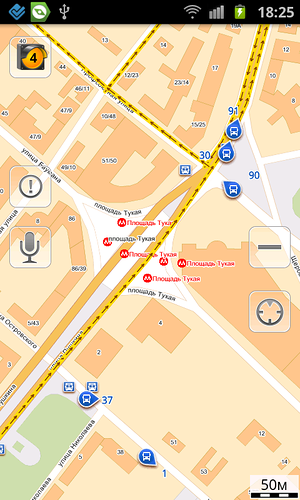
\includegraphics[height=0.7\textheight]{yakazan.png}

		Buses of the city of Kazan in real time.
	\end{columns}
}

\frame{
	\frametitle{The general architecture}
	\center{
		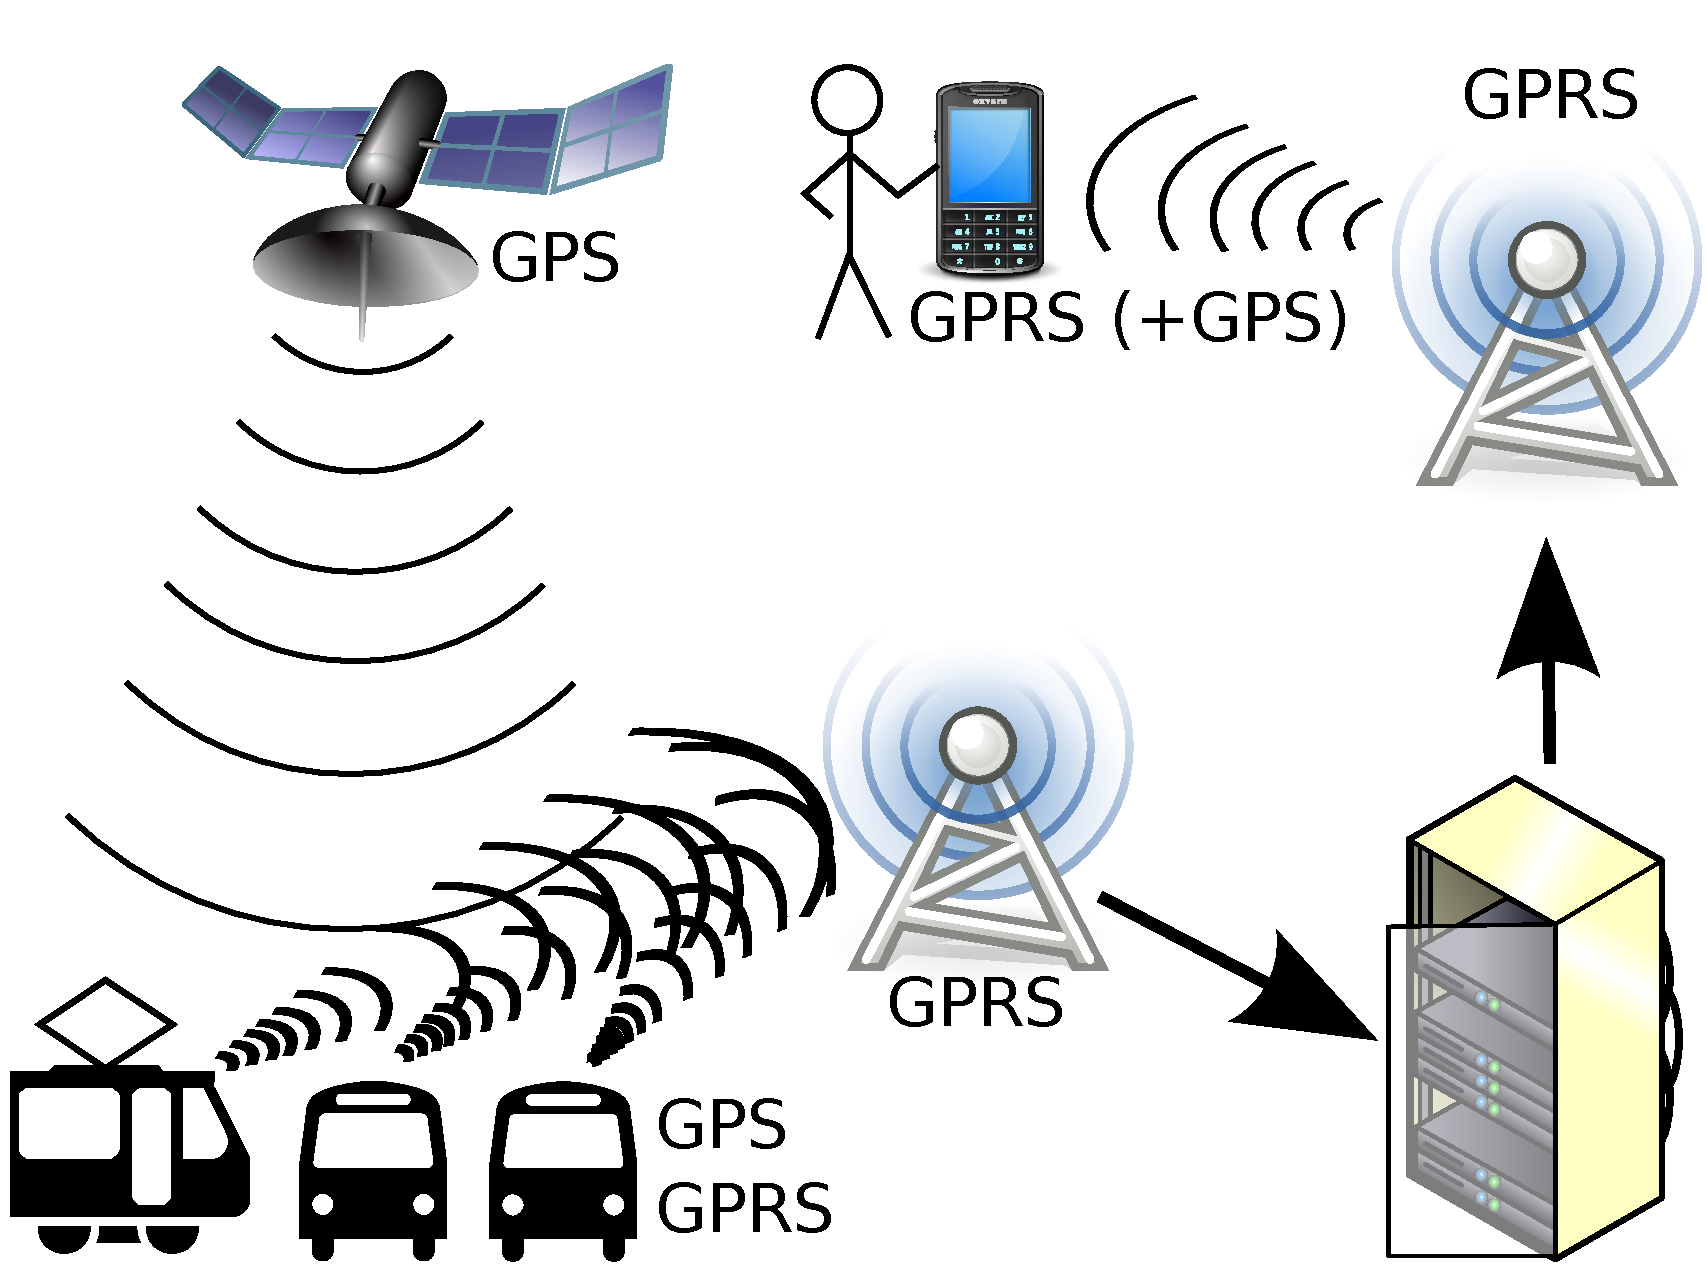
\includegraphics[width=0.9\textwidth]{general-arch-pict.pdf}
	}
}

\frame{
	\frametitle{Existing positioning methods}
	\begin{columns}[c]
		\column{0.5\textwidth}
		Satellite navigation
		\begin{itemize}
			\item
				Satellites
			\item
				Based on signal delay
			\item
				Very precise, simple formulas
			\item
				1 -- 50 meters of error
		\end{itemize}
		\column{0.5\textwidth}
		Cellular
		\begin{itemize}
			\item
				GSM cells
			\item
				Based on signal levels
			\item
				Not precise, sophisticated methods
			\item
				10 -- 500 meters of error
		\end{itemize}
	\end{columns}
}
\frame{
	\frametitle{Hypothesis}
	Over-extrapolation affects the precision of cell-based positioning
	\begin{columns}[T]
		\column{0.5\textwidth}
		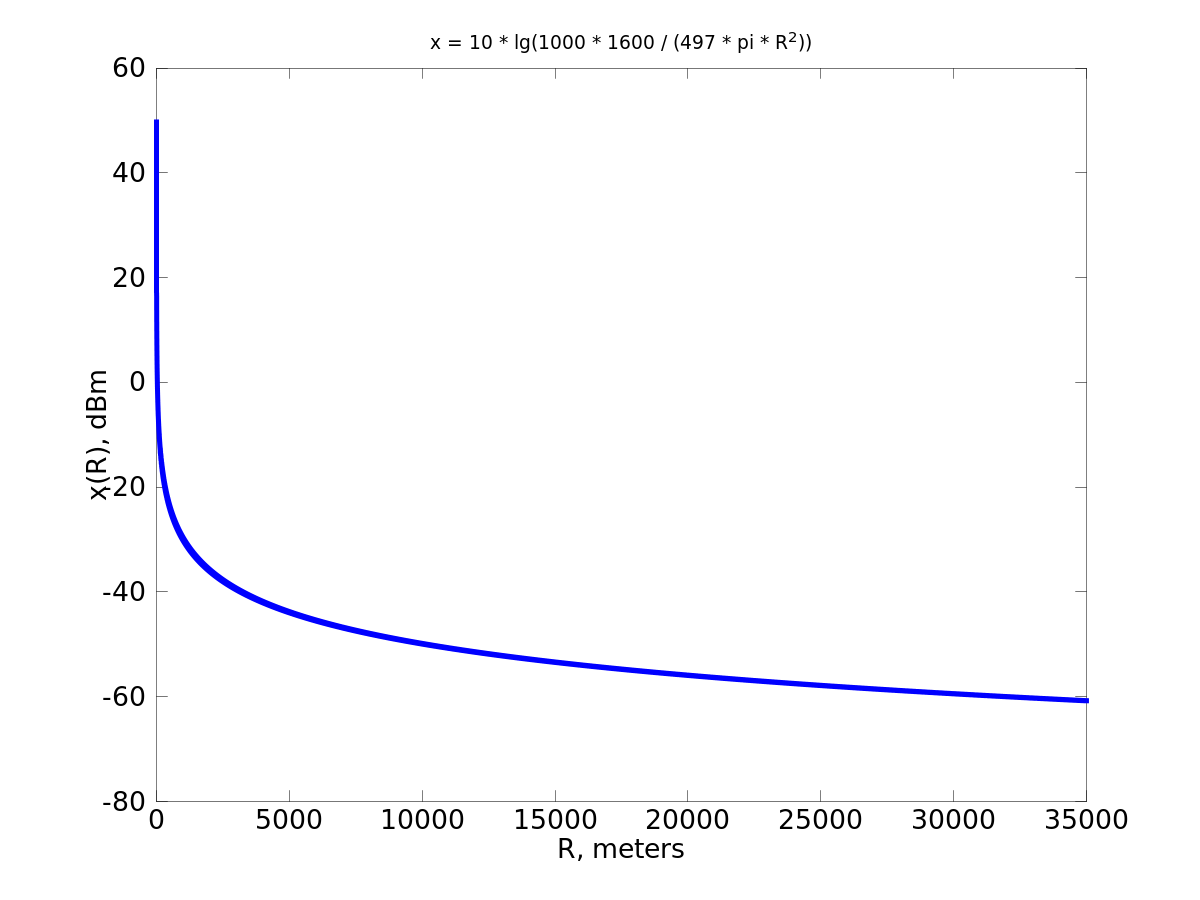
\includegraphics[width=1\linewidth]{bs40wdbm-contrast.png}\\
		Theoretical estimate of signal attenuation
		\column{0.5\textwidth}
		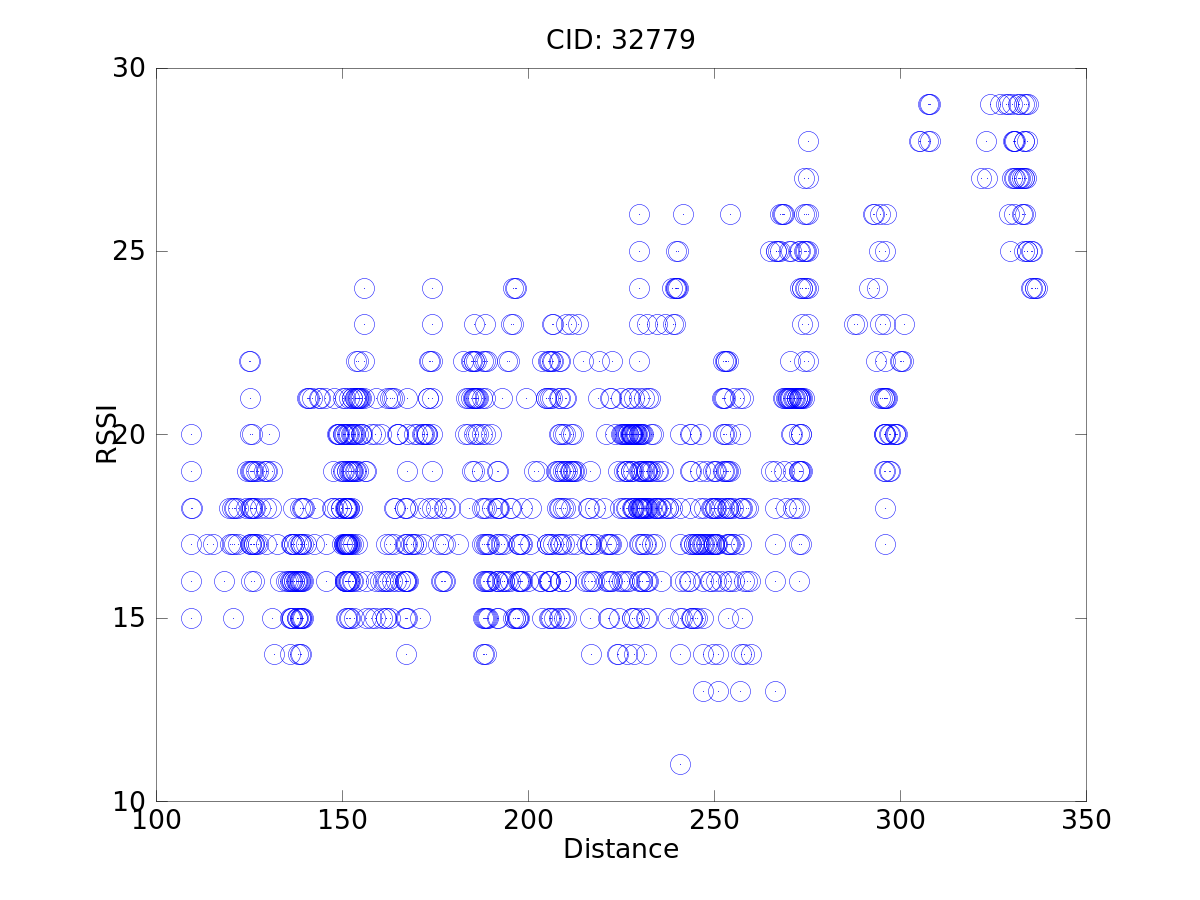
\includegraphics[width=1\linewidth]{cell32779raw-contrast.png}\\
		Experimental data
	\end{columns}
}

\frame{
	\frametitle{Public transportation}
	A predefined route:
	\begin{itemize}
		\item
			Makes the problem one-dimensional
		\item
			Allows us to obtain more statistical data
	\end{itemize}
}

\frame{
	\frametitle{Existing statistical methods}
	\begin{tabular}{|p{0.4\textwidth}|p{0.25\textwidth}|p{0.25\textwidth}|}
		\hline
		{\bf{}Parameter} & {\bf{}Mahalanobis distance} & {\bf{}Bayesian classifier} \\
		\hline
		Continuousness of an argument & - & - \\
		\hline
		Continuousness of a value & + & - \\
		\hline
		Resistance to anomalies & - & + \\
		\hline
	\end{tabular}
}

\frame{
	\frametitle{My algorithm}
	The algorithm being proposed:
	\begin{enumerate}
		\item
			Considers the continuousness of a random value -- a signal level;
		\item
			Considers data from adjacent points;
		\item
			Is resistant to anomalies.
	\end{enumerate}
	How does it work?
}

\frame{
	\frametitle{Selecting from a datbase}
	\begin{columns}[T]
		\begin{column}{0.75\textwidth}
			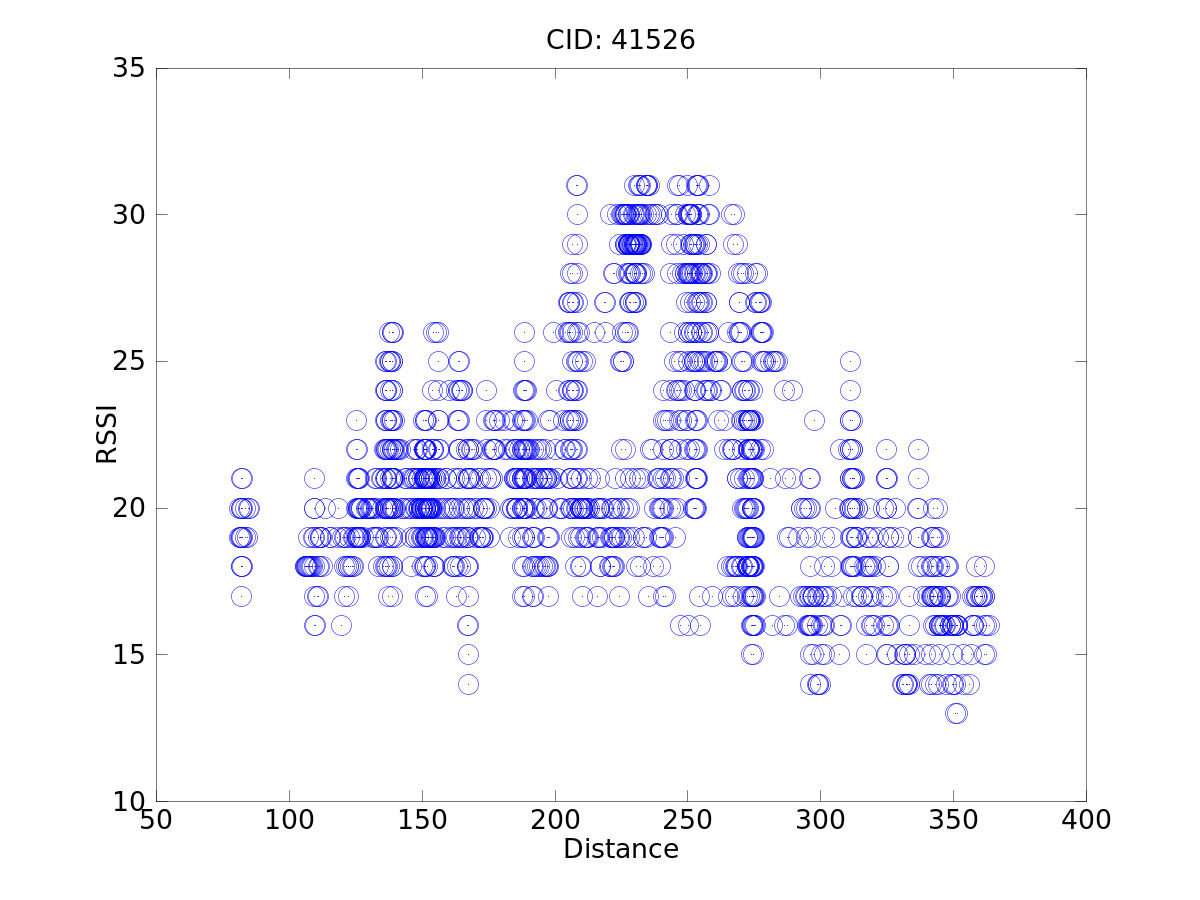
\includegraphics[width=0.9\textwidth]{cell41526raw-contrast.png}

			\hspace{1em}
			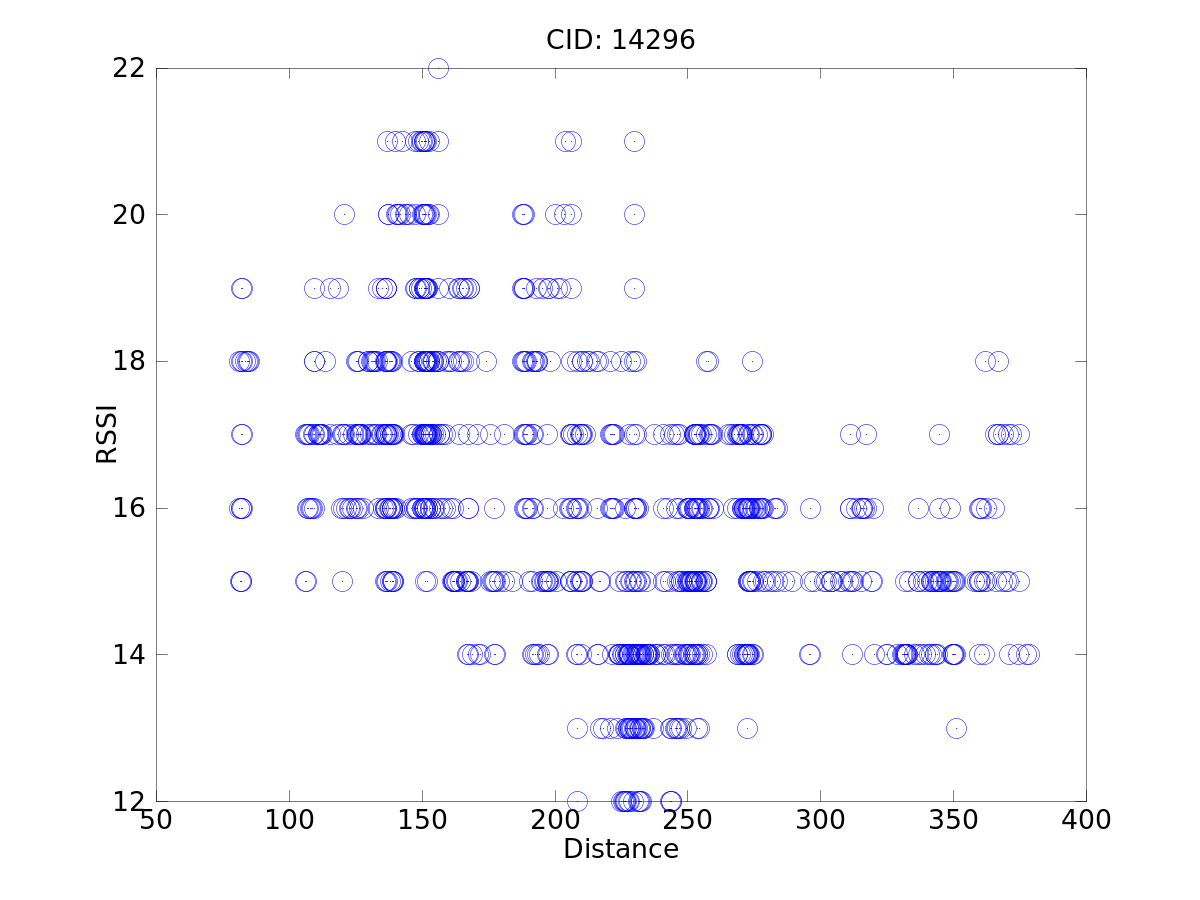
\includegraphics[width=0.37\textwidth]{cell14296raw-contrast.png}
			\hspace{1em}
			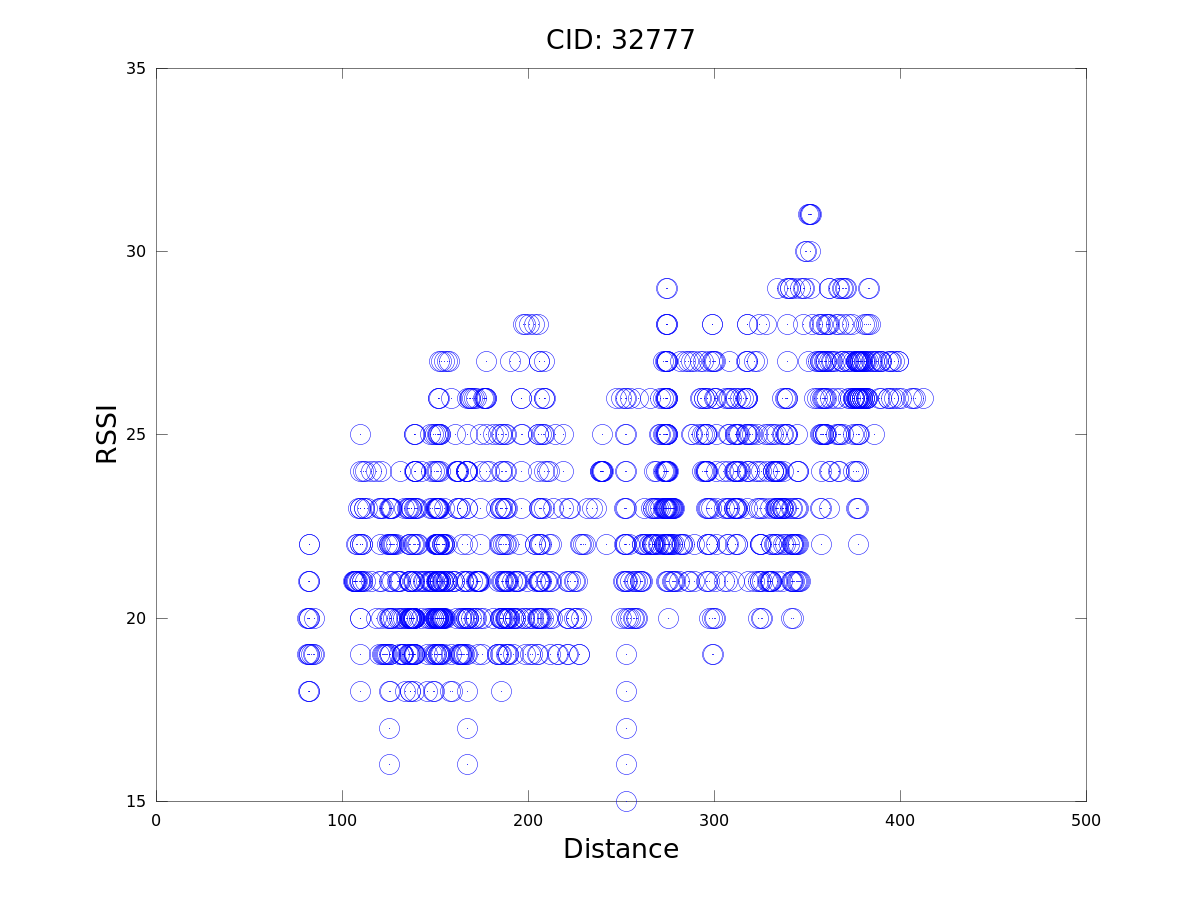
\includegraphics[width=0.37\textwidth]{cell32777raw-contrast.png}
			\end{column}

		\begin{column}{0.32\textwidth}
			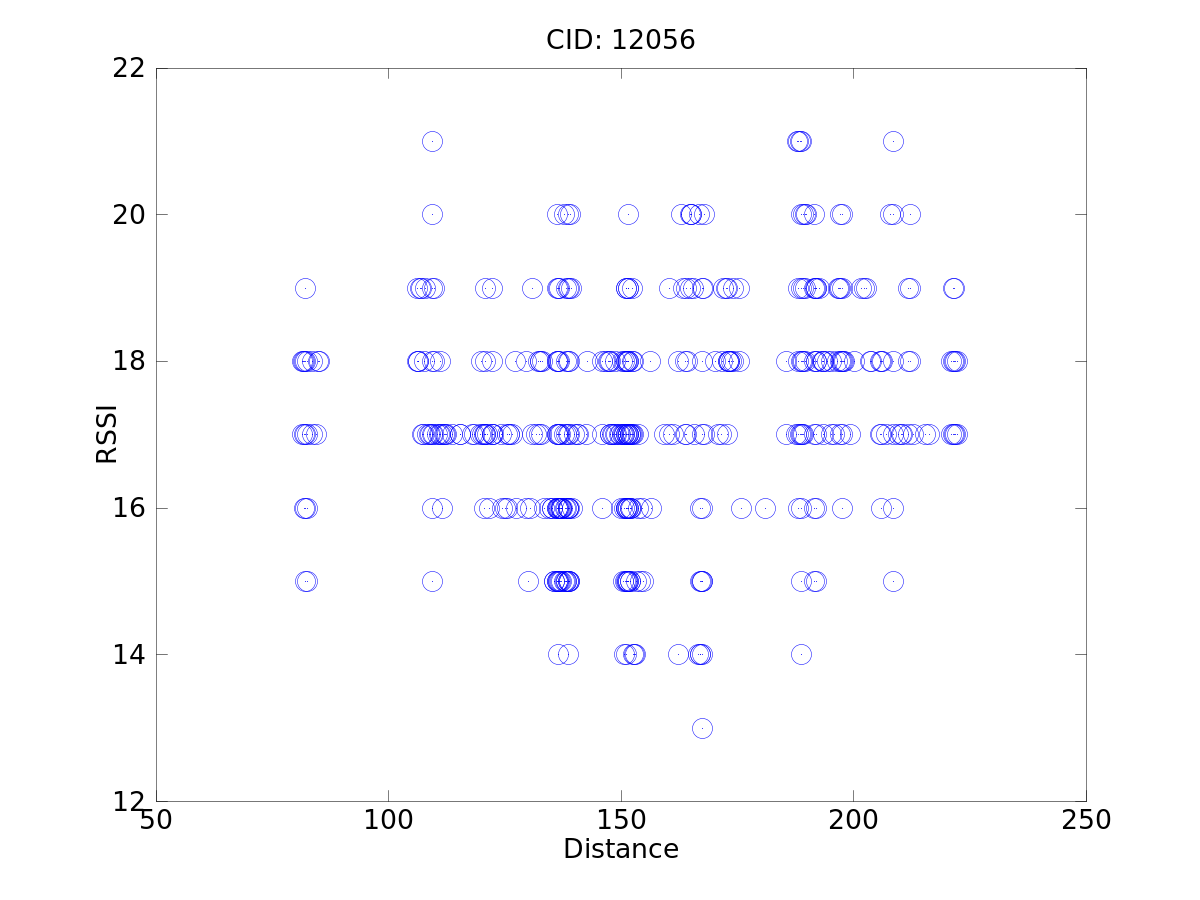
\includegraphics[width=0.95\textwidth]{cell12056raw-contrast.png}

			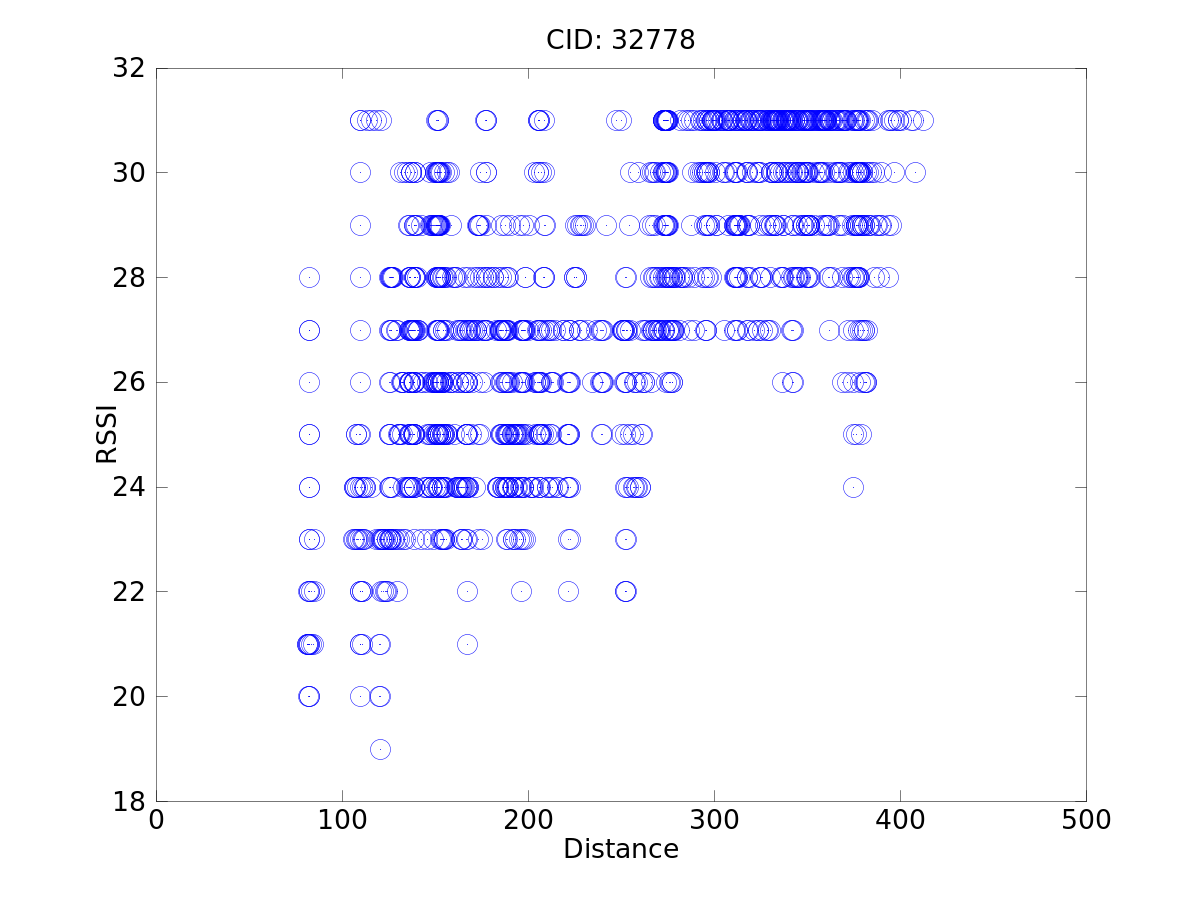
\includegraphics[width=0.95\textwidth]{cell32778raw-contrast.png}
	
			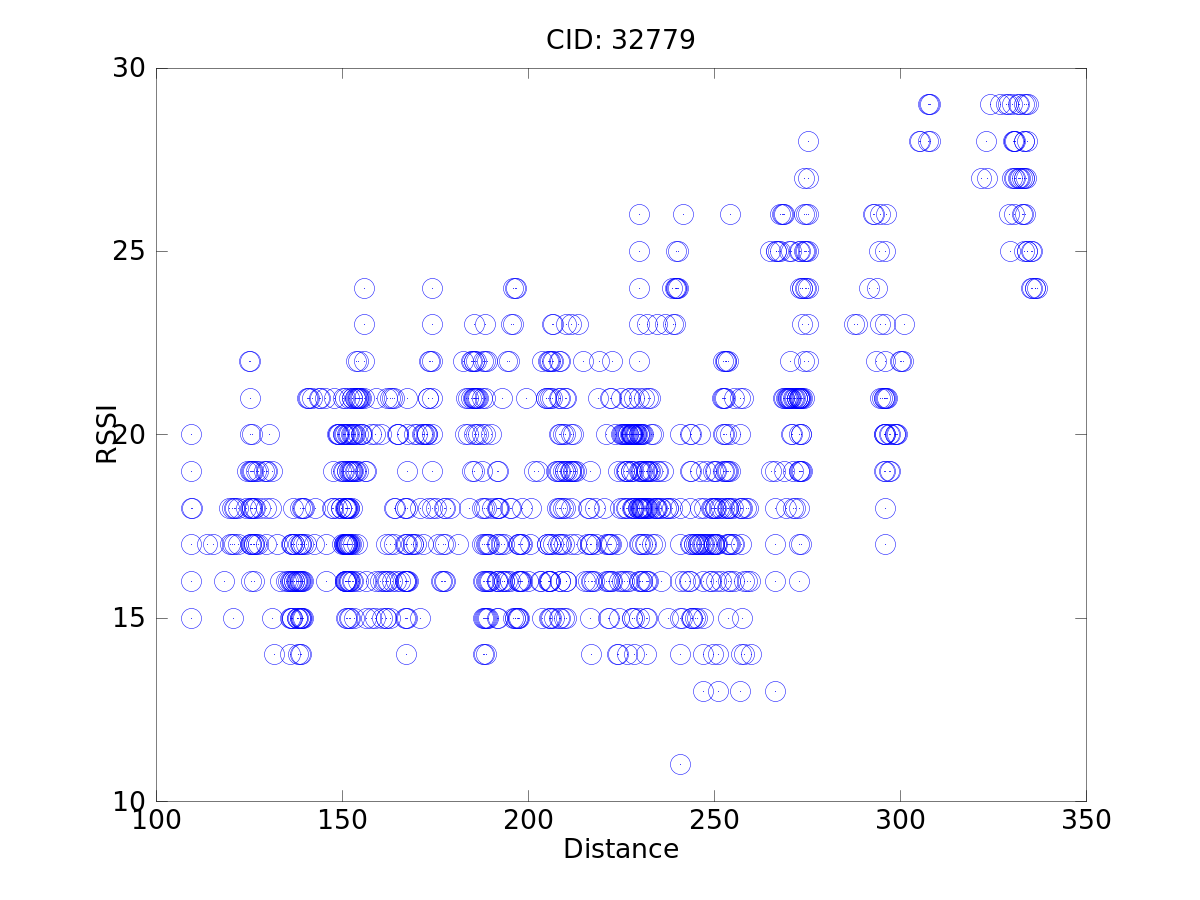
\includegraphics[width=0.95\textwidth]{cell32779raw-contrast.png}
		\end{column}
	\end{columns}
}

\frame{
	\frametitle{Approximation}
	\begin{columns}[T]
		\begin{column}{0.75\textwidth}
			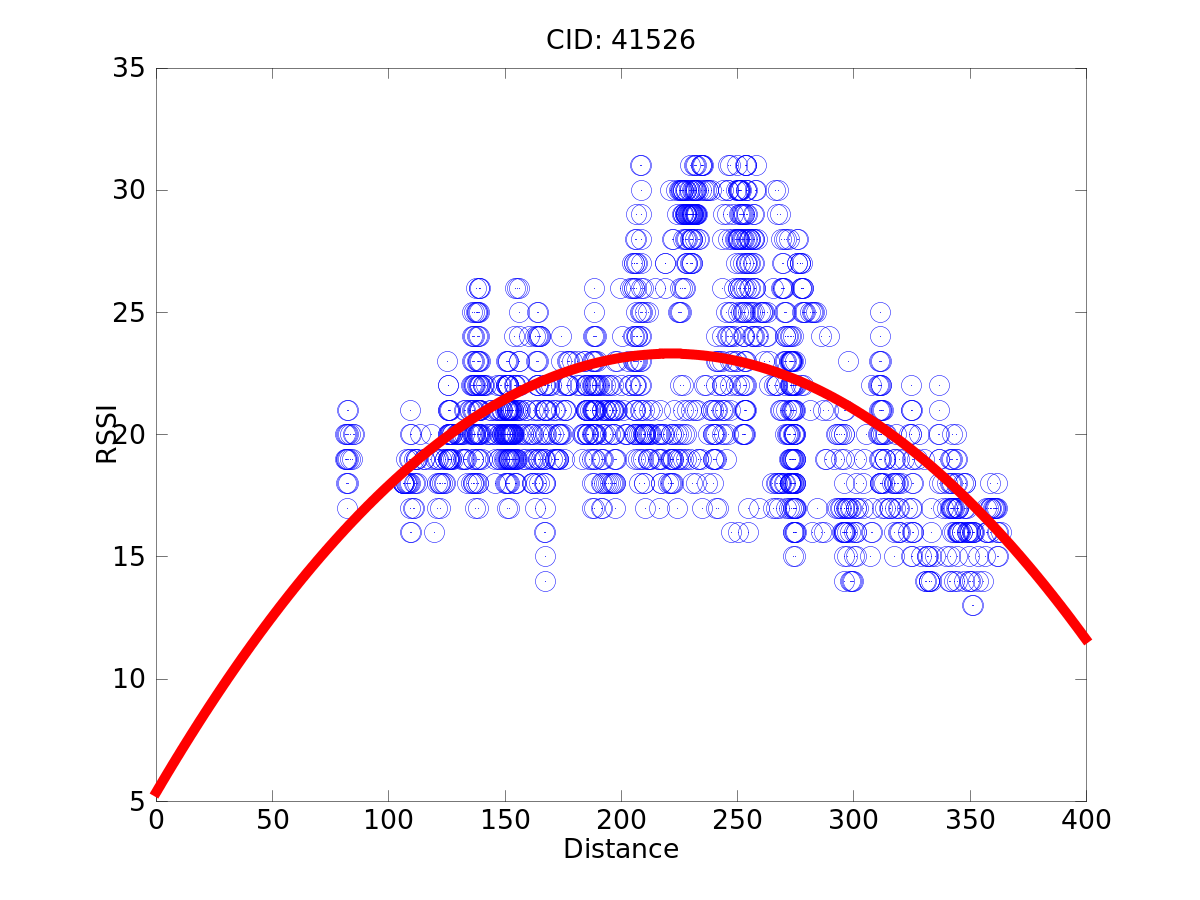
\includegraphics[width=0.9\textwidth]{cell41526inter-contrast.png}

			\hspace{1em}
			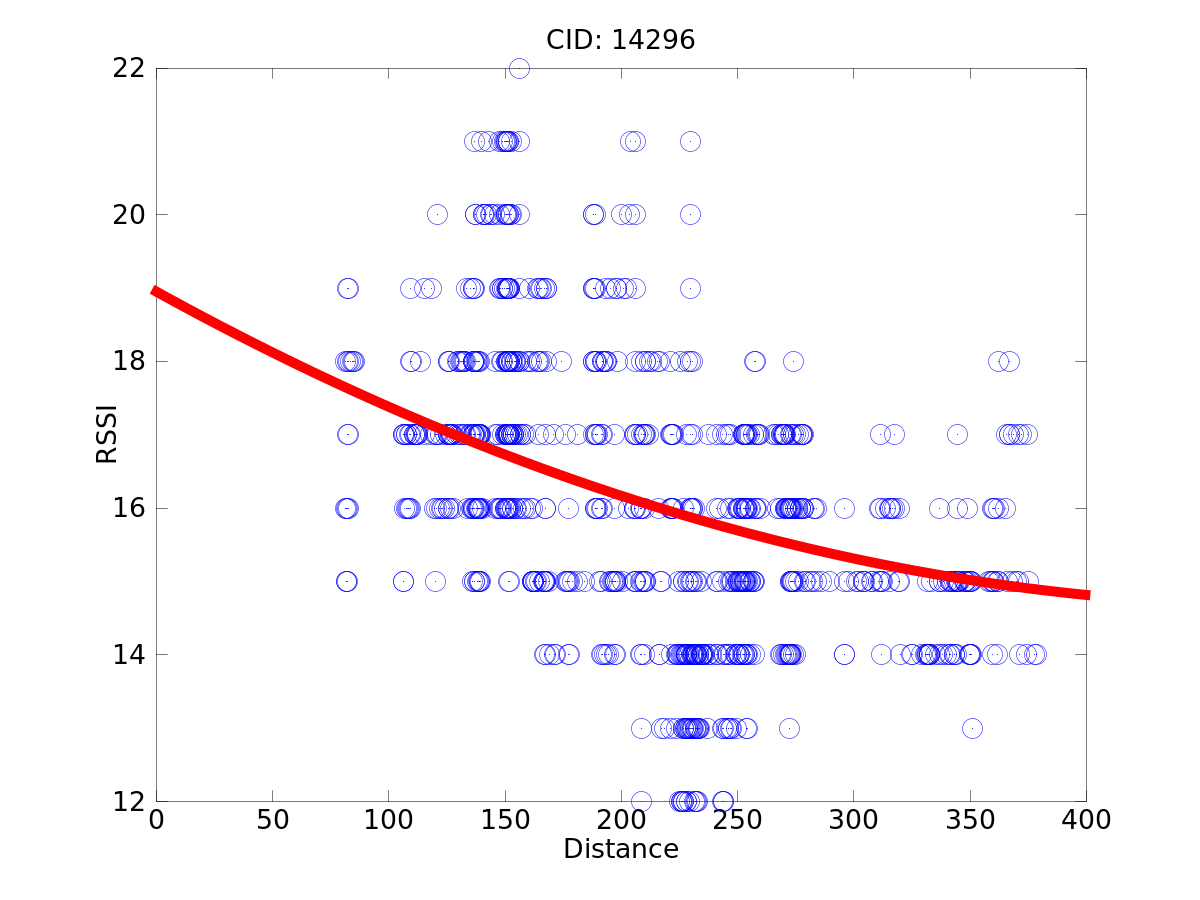
\includegraphics[width=0.37\textwidth]{cell14296inter-contrast.png}
			\hspace{1em}
			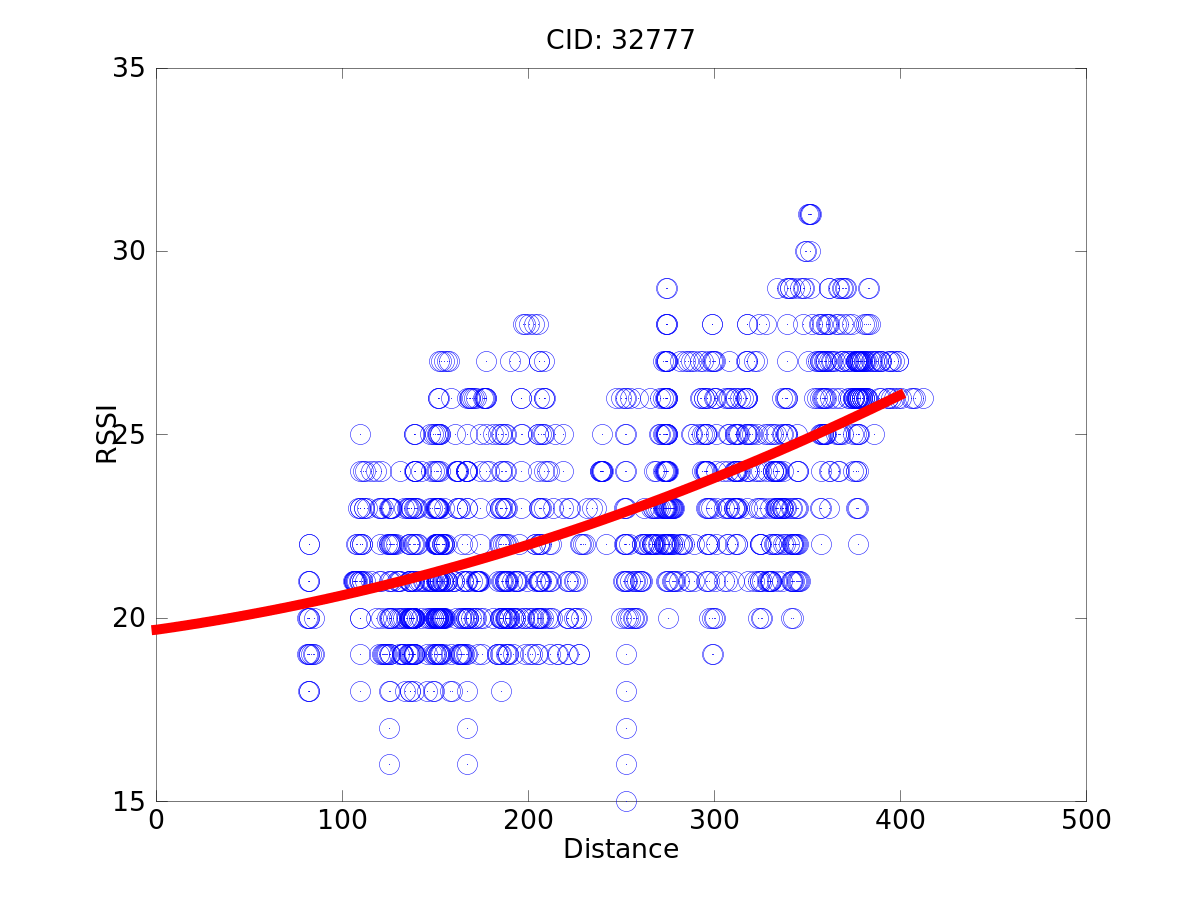
\includegraphics[width=0.37\textwidth]{cell32777inter-contrast.png}
			\end{column}

		\begin{column}{0.32\textwidth}
			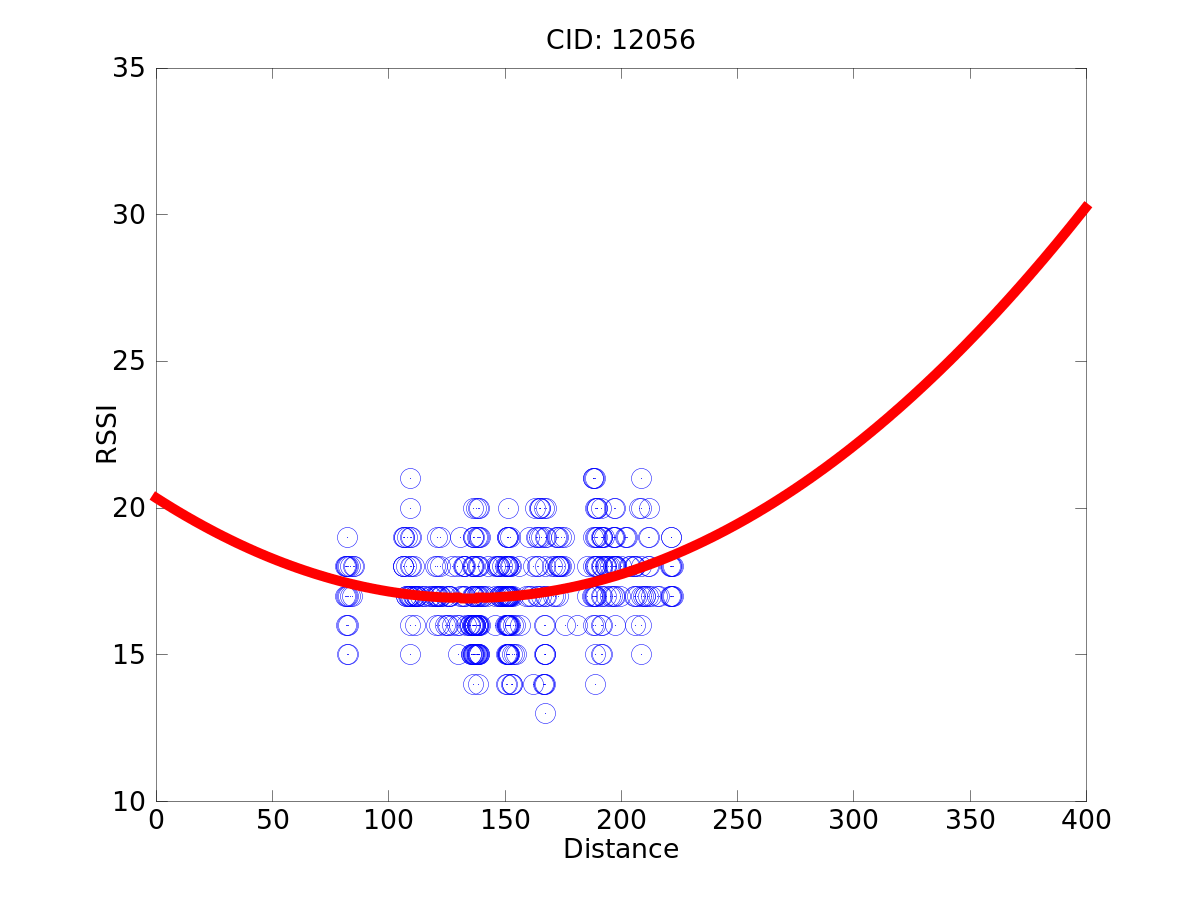
\includegraphics[width=0.95\textwidth]{cell12056inter-contrast.png}

			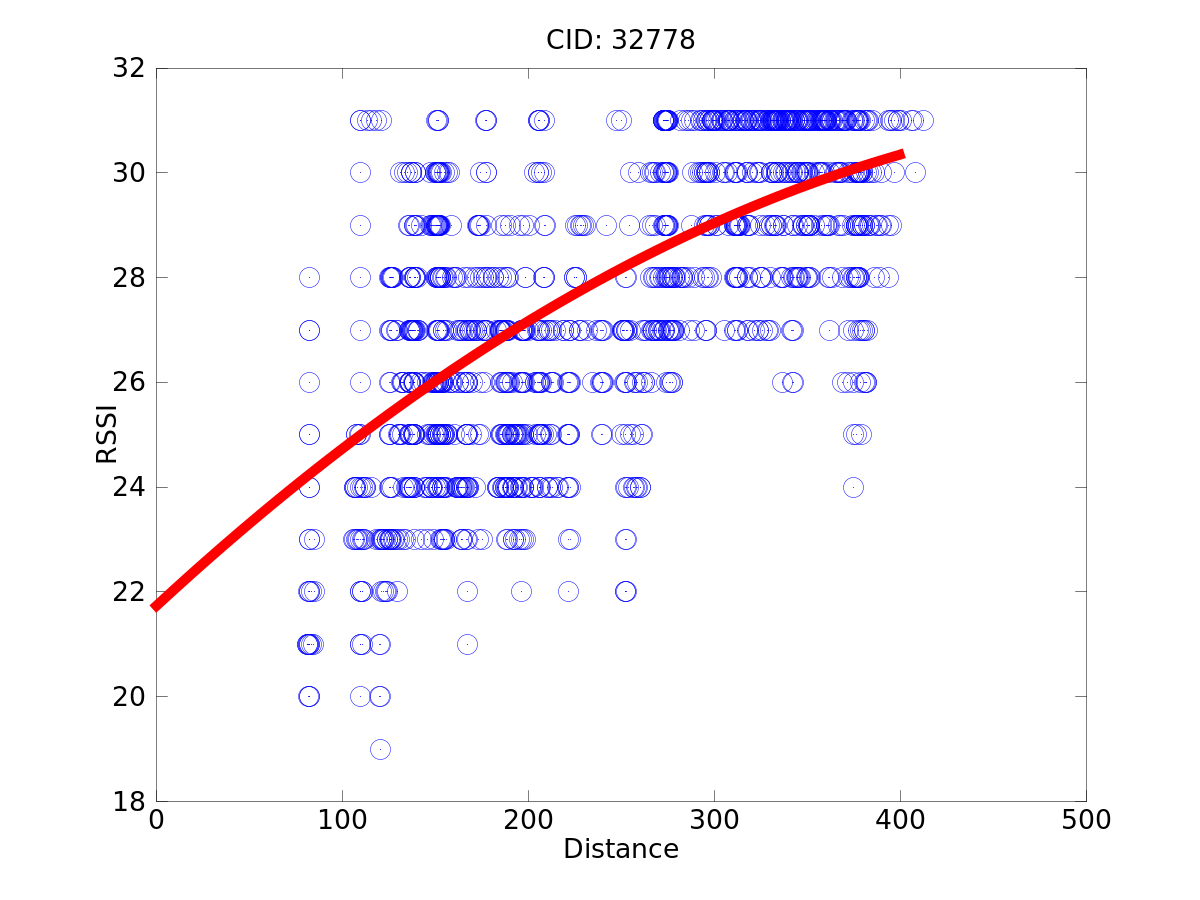
\includegraphics[width=0.95\textwidth]{cell32778inter-contrast.png}
	
			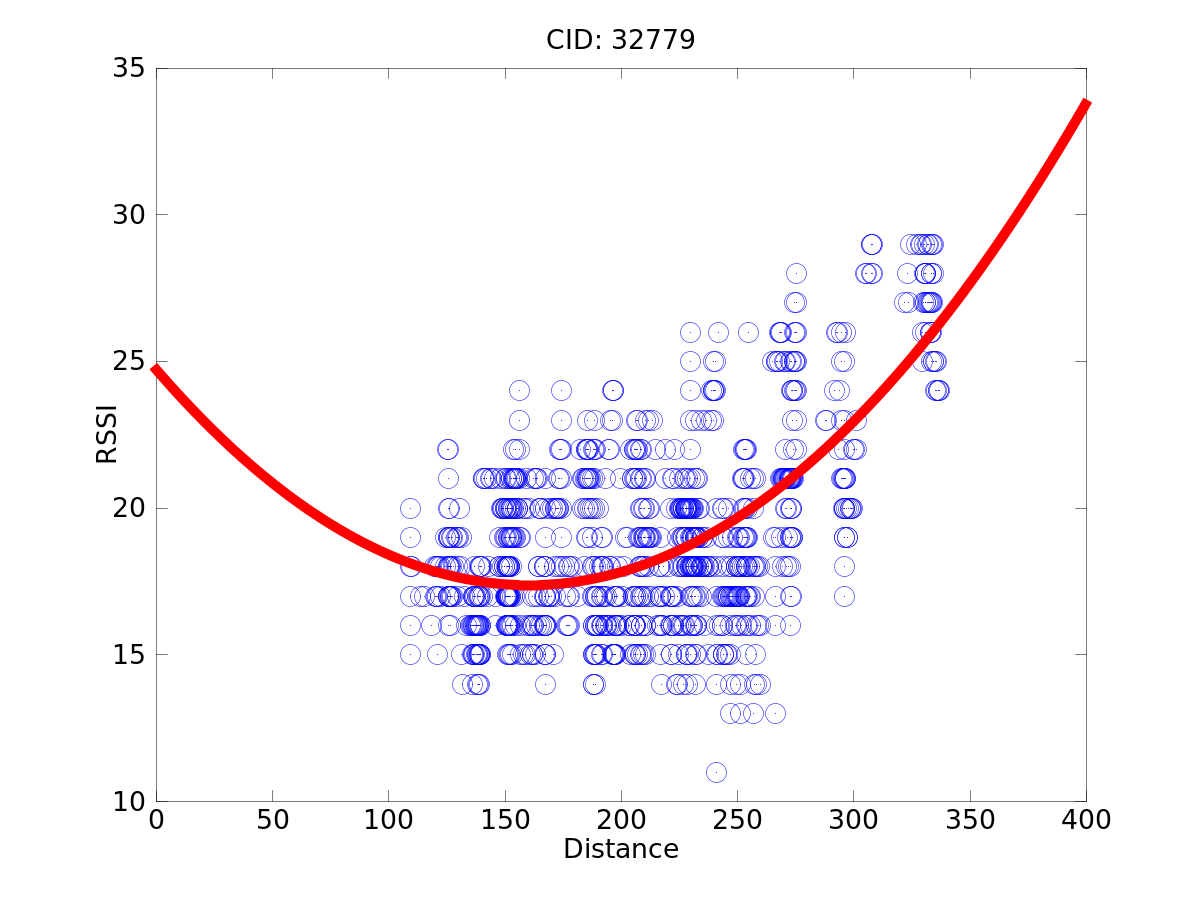
\includegraphics[width=0.95\textwidth]{cell32779inter-contrast.png}
		\end{column}
	\end{columns}

}

\frame{
	\frametitle{Pseudo-probability density}
	Requirements:
	\begin{enumerate}
		\item
			$\forall_{f(x), y}P(f(x), y)\in(0,1]$
		\item
			$\forall_{f(x), y}f(x) = y\Leftrightarrow{}P(f(x),y) = 1$
		\item
			$\lim\limits_{|f(x)-y|\to\infty}P(f(x),y) = 0$
	\end{enumerate}
	Implementation:
	\begin{equation}
		P(f(x), y) = \frac{1}{1+(f(x)-y)^2}
		\nonumber
		\label{eq:pseudop}
	\end{equation}
}
\frame{
	\frametitle{Calculating pseudo-density}
	\begin{columns}[T]
		\begin{column}{0.75\textwidth}
			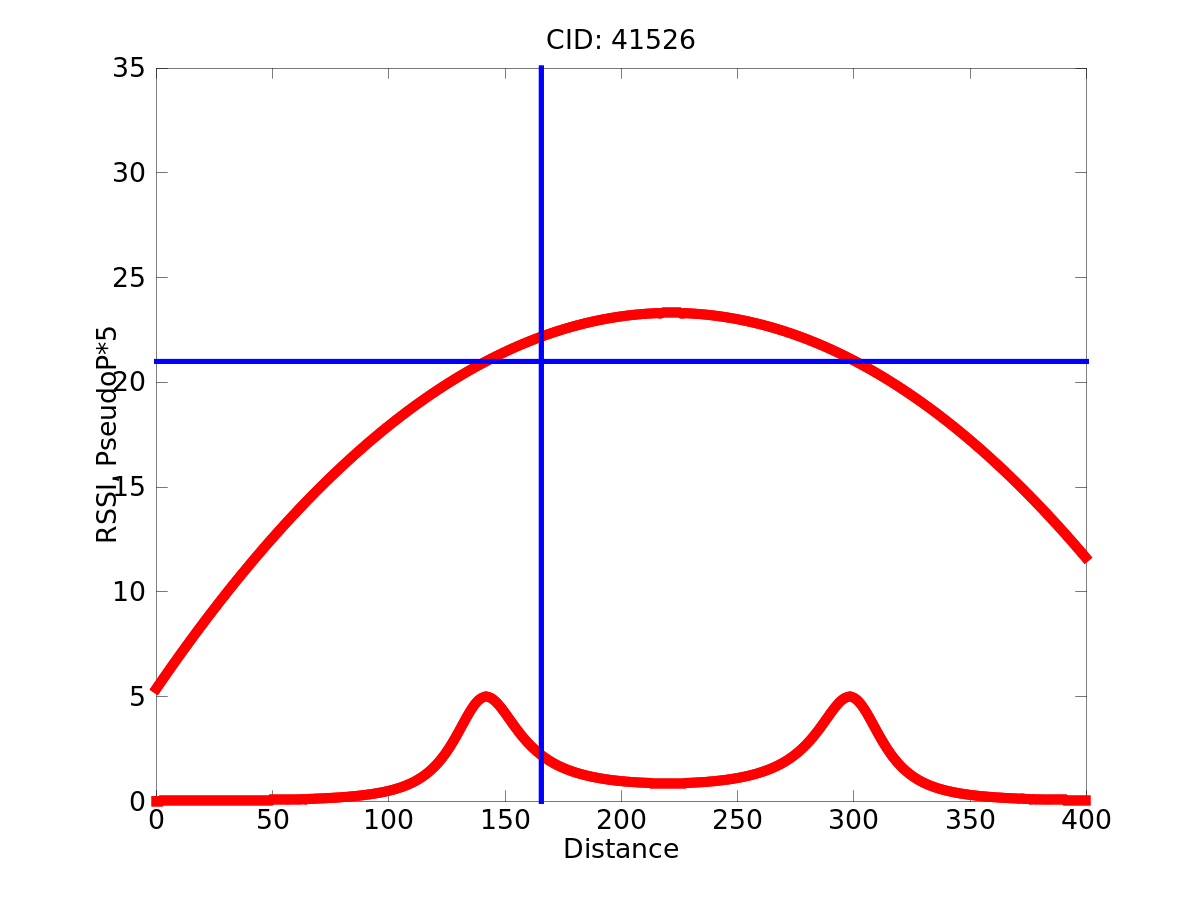
\includegraphics[width=0.9\textwidth]{cell41526pseudop-contrast.png}

			\hspace{1em}
			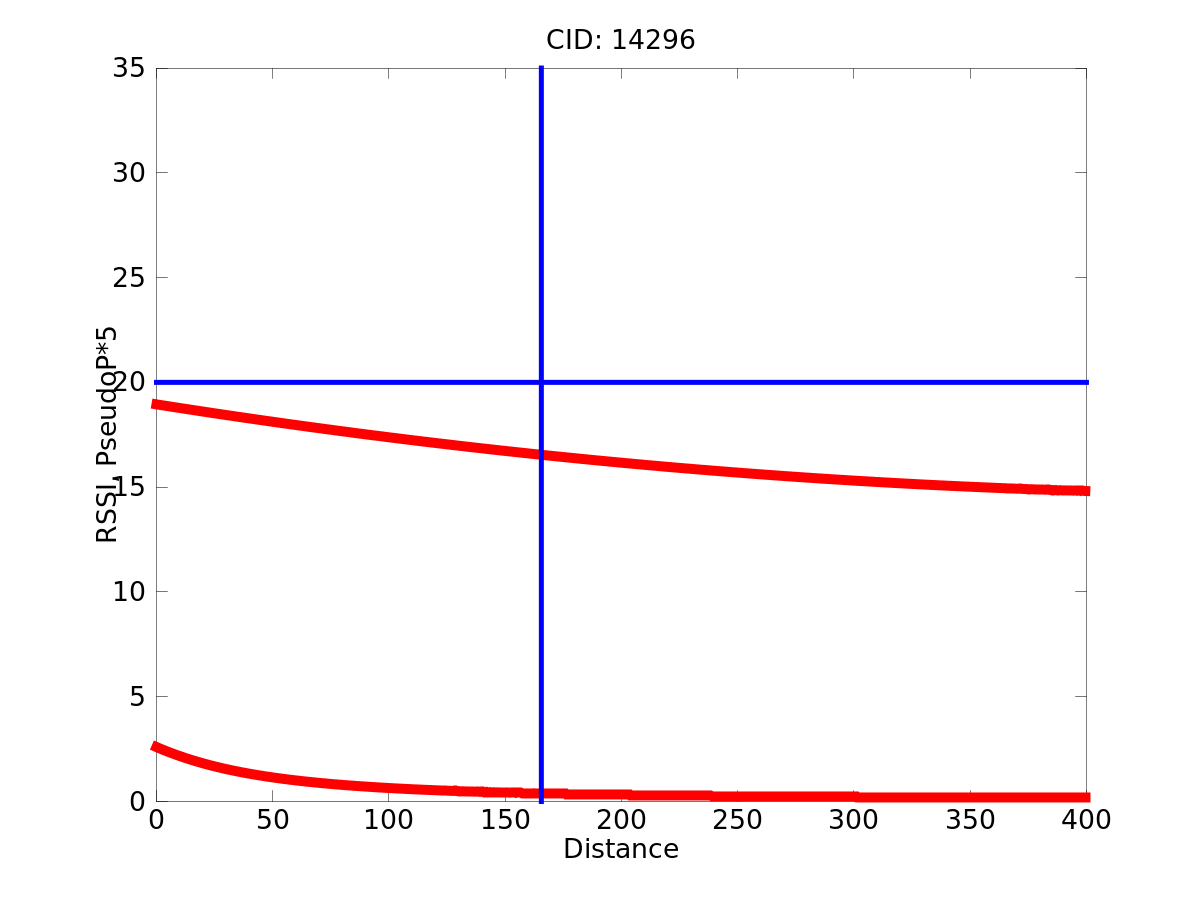
\includegraphics[width=0.37\textwidth]{cell14296pseudop-contrast.png}
			\hspace{1em}
			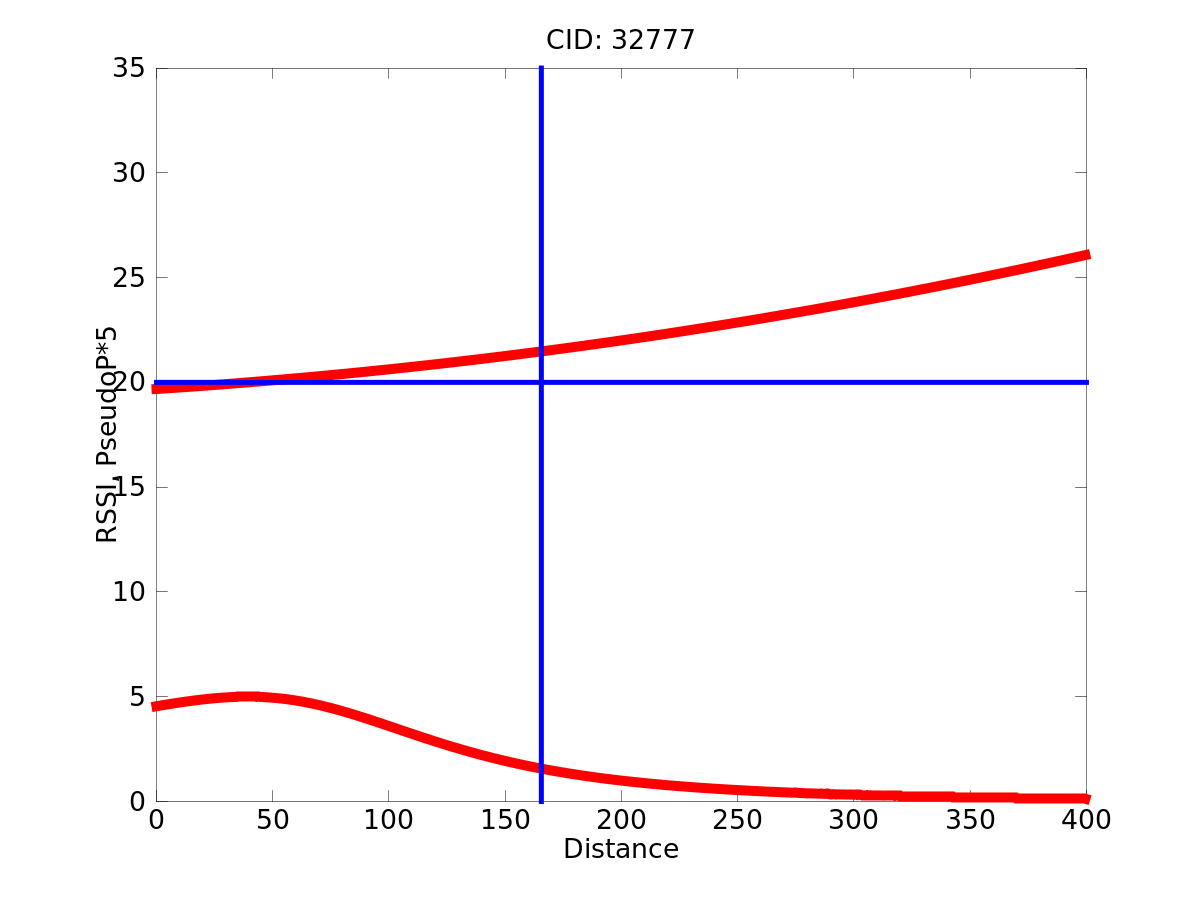
\includegraphics[width=0.37\textwidth]{cell32777pseudop-contrast.png}
			\end{column}

		\begin{column}{0.32\textwidth}
			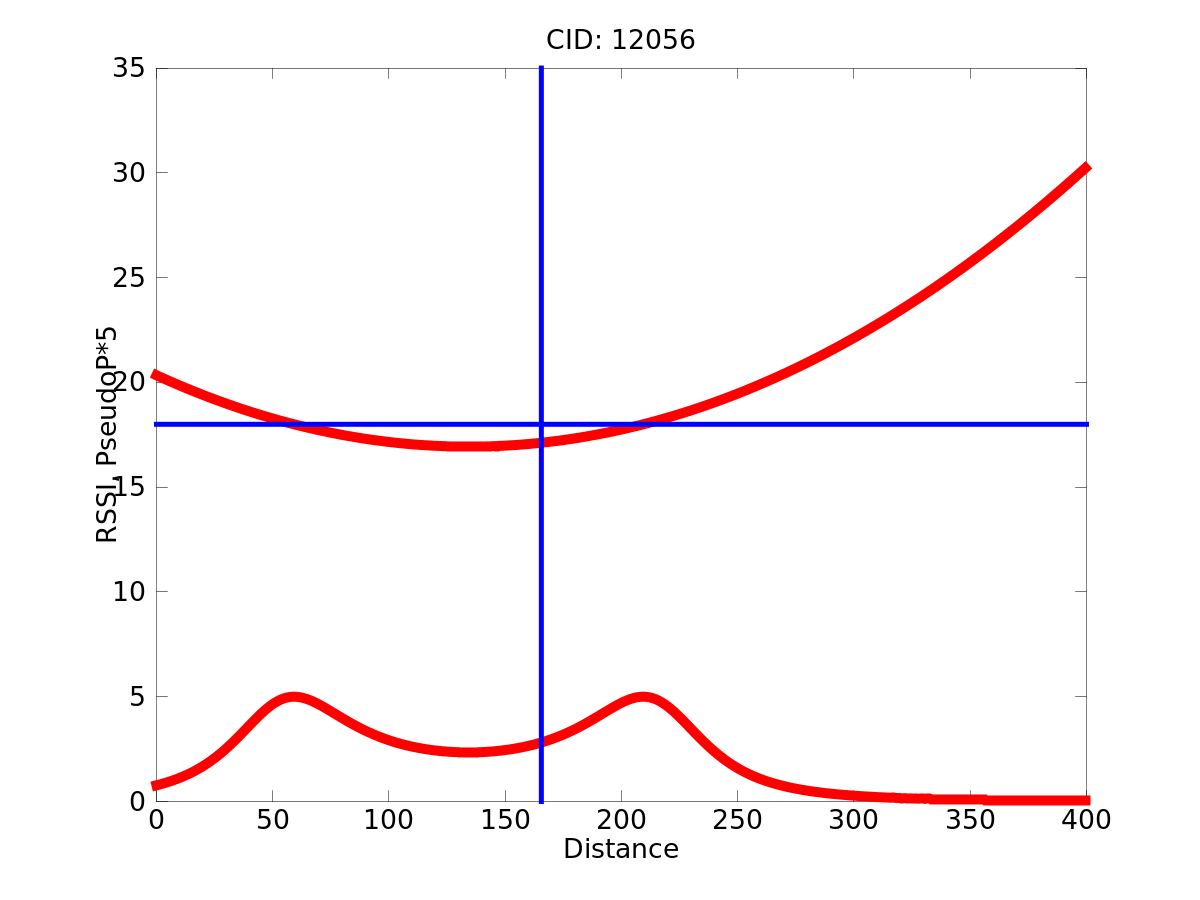
\includegraphics[width=0.95\textwidth]{cell12056pseudop-contrast.png}

			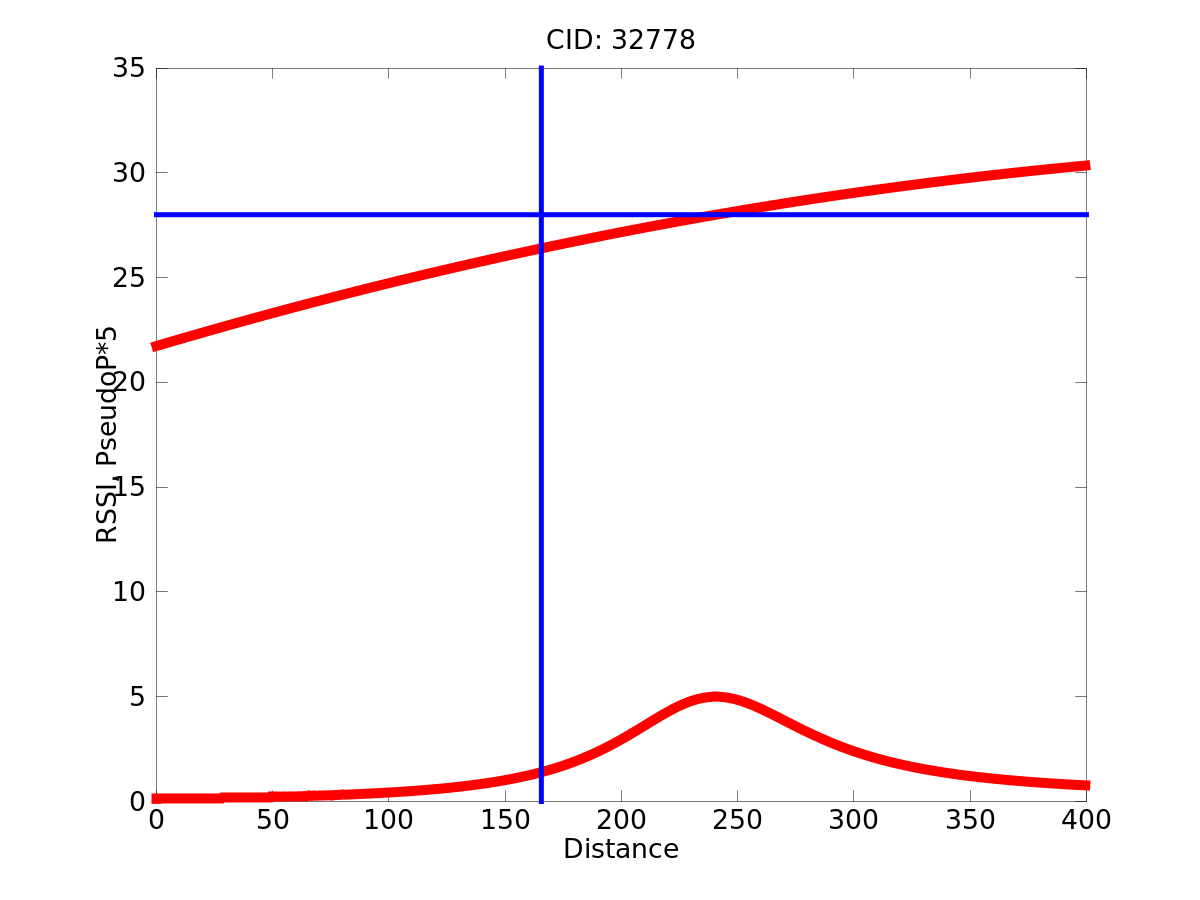
\includegraphics[width=0.95\textwidth]{cell32778pseudop-contrast.png}
	
			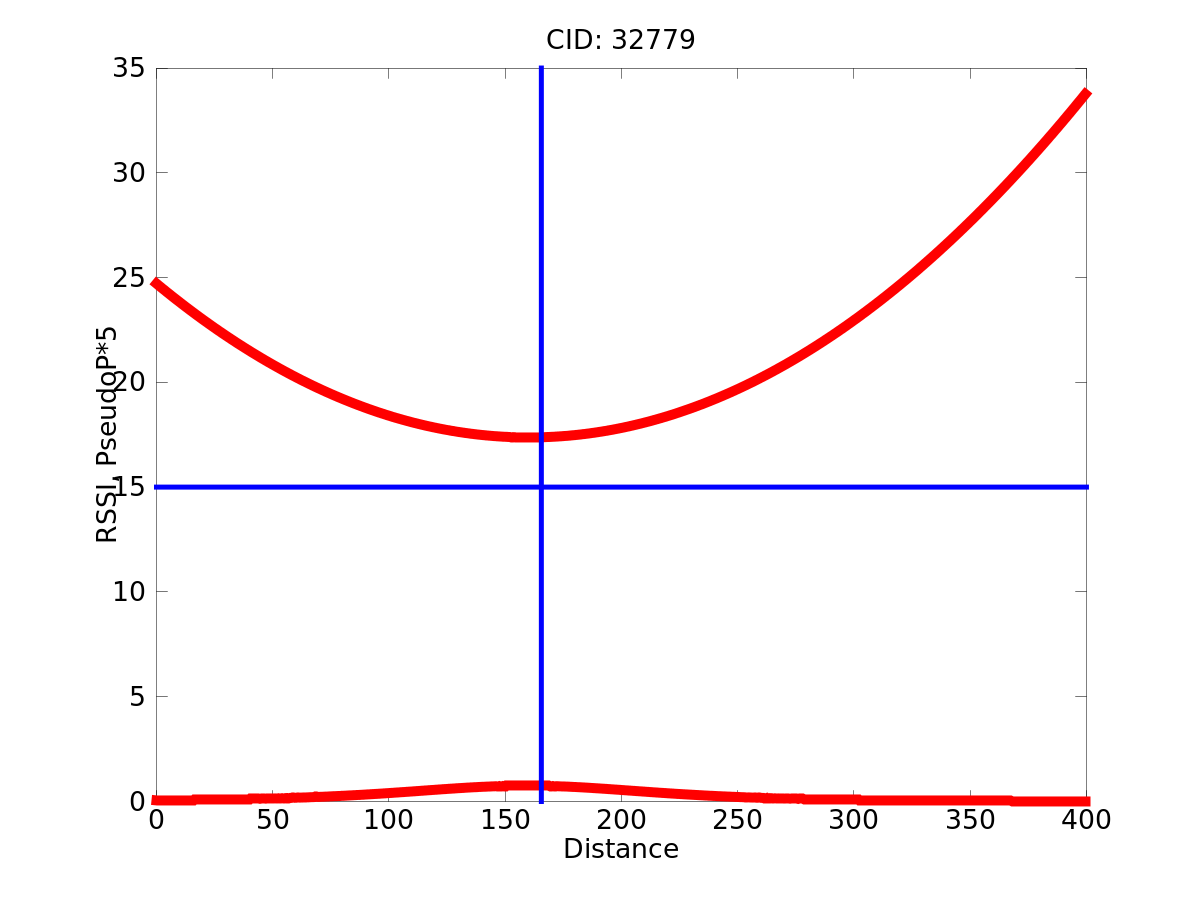
\includegraphics[width=0.95\textwidth]{cell32779pseudop-contrast.png}
		\end{column}
	\end{columns}

}

\frame{
	\frametitle{Resulting pseudo-density}
	Result: 143 meters, actual position (according to GPS): 165,5 метров.

	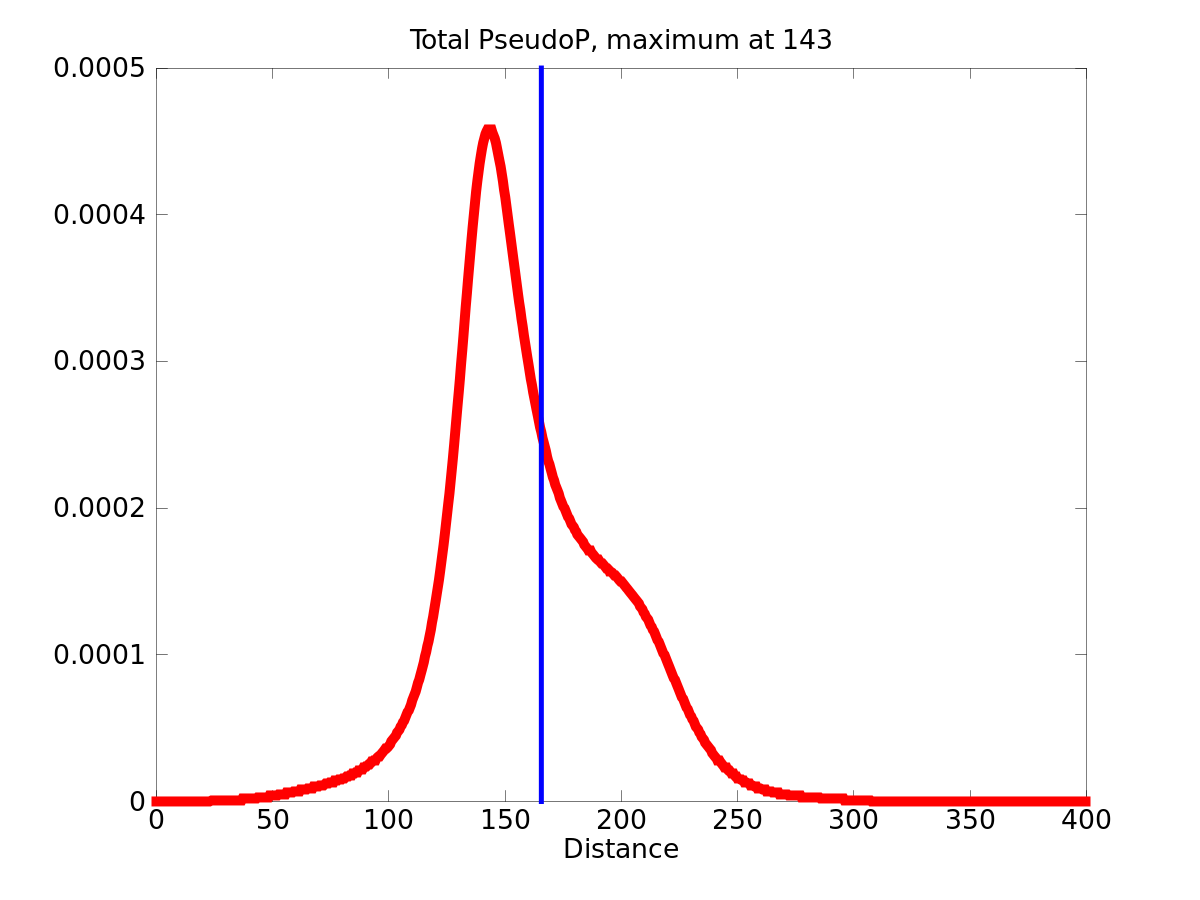
\includegraphics[height=0.8\textheight]{totalpseudop-contrast.png}
}

\frame{
	\frametitle{Architecture}
	\centerline{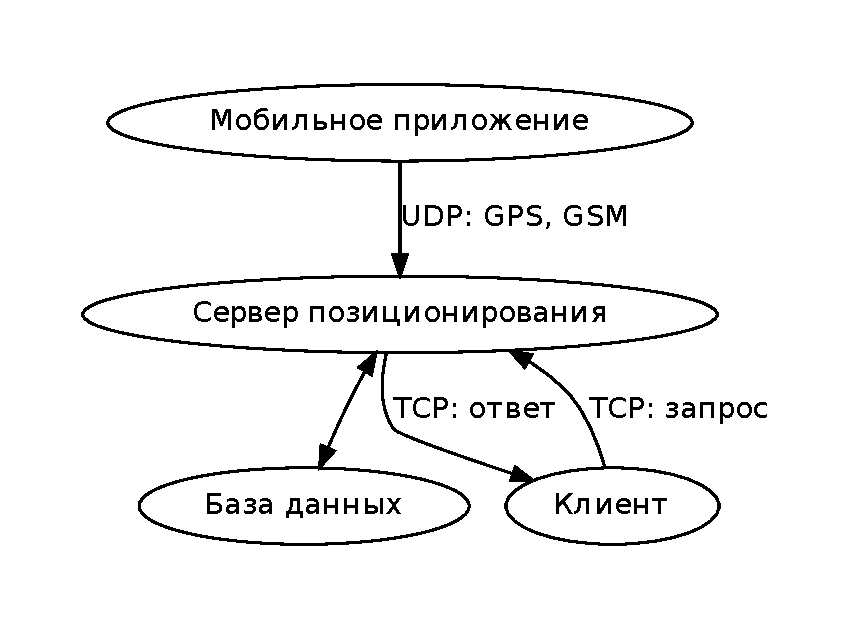
\includegraphics[height=0.8\textheight]{general-arch.pdf}}
}

\frame{
	\frametitle{Testing}
	\centerline{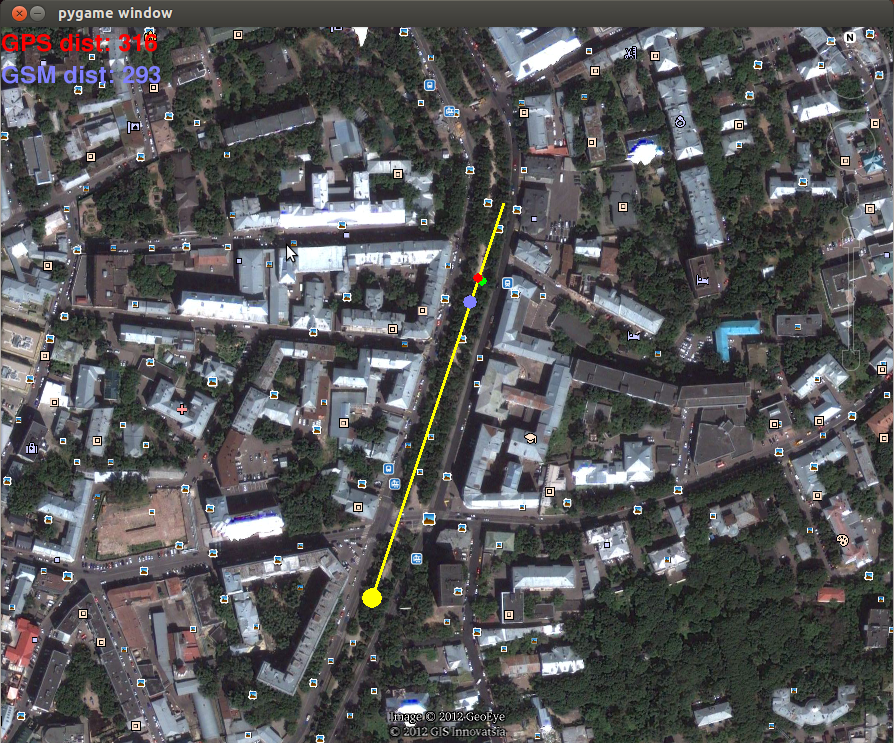
\includegraphics[height=0.8\textheight]{gfront-gsm-mode.png}}
}

\frame{
	\frametitle{Histogram of errors}
	176 experiments, the mean value of errors: 49 meters.

	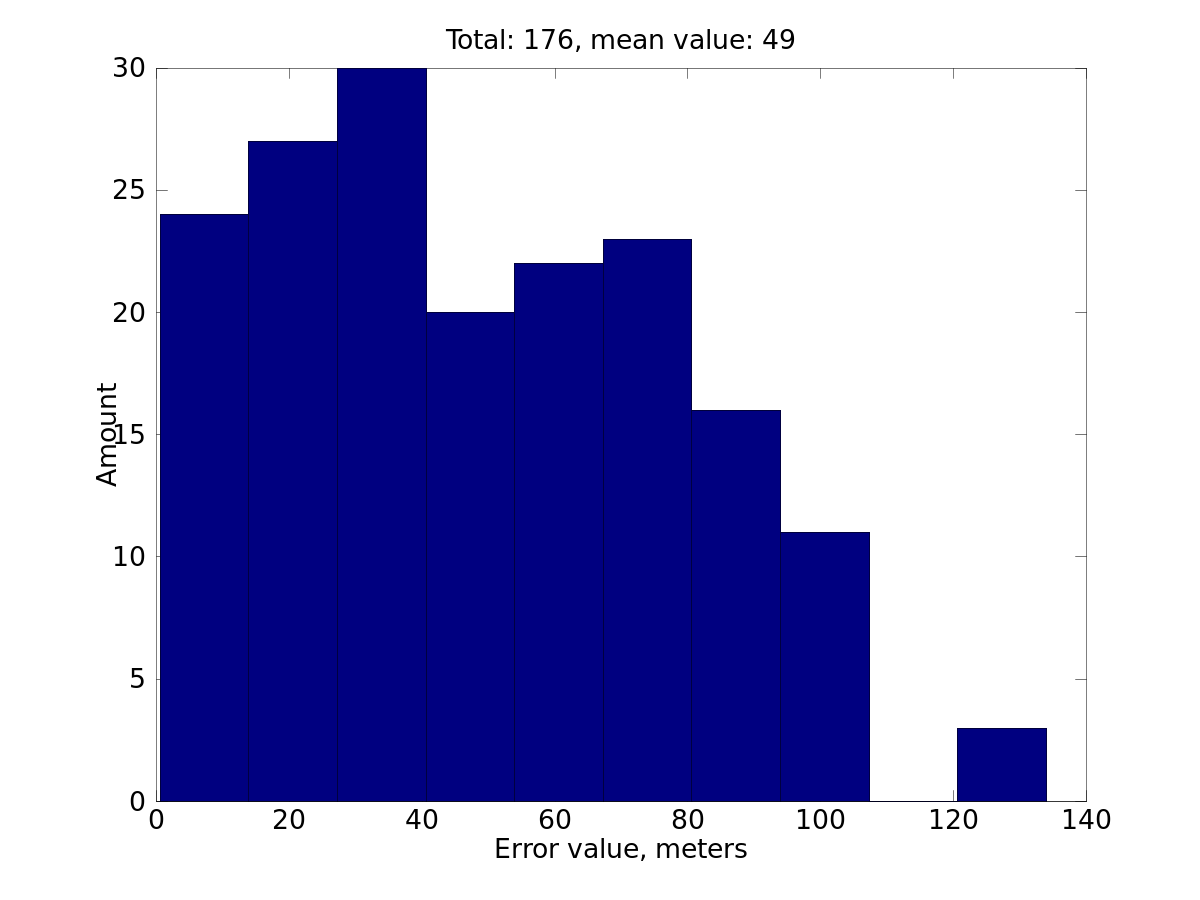
\includegraphics[height=0.8\textheight]{errhist-contrast.png}
}

\begin{frame}[fragile]
	\frametitle{Comparison}
	\begin{tabular}{|p{0.2\textwidth}|p{0.2\textwidth}|p{0.23\textwidth}|p{0.2\textwidth}|}
		\hline
		{\bf{}Parameter} & {\bf{}GPS} & {\bf{}Triangulation} & {\bf{}My algorithm} \\
		\hline
		Precision, meters & 10 & 200 & 50 \\
		\hline
		Cost & GPS+GSM & GSM & GSM \\
		\hline
		Coverage & Worldwide & Citywide & Route-wide \\
		\hline
	\end{tabular}
\end{frame}

\frame{
	\frametitle{Analyzing results}
\begin{figure}[h]
	\begin{columns}[T]
		\column{0.45\textwidth}
			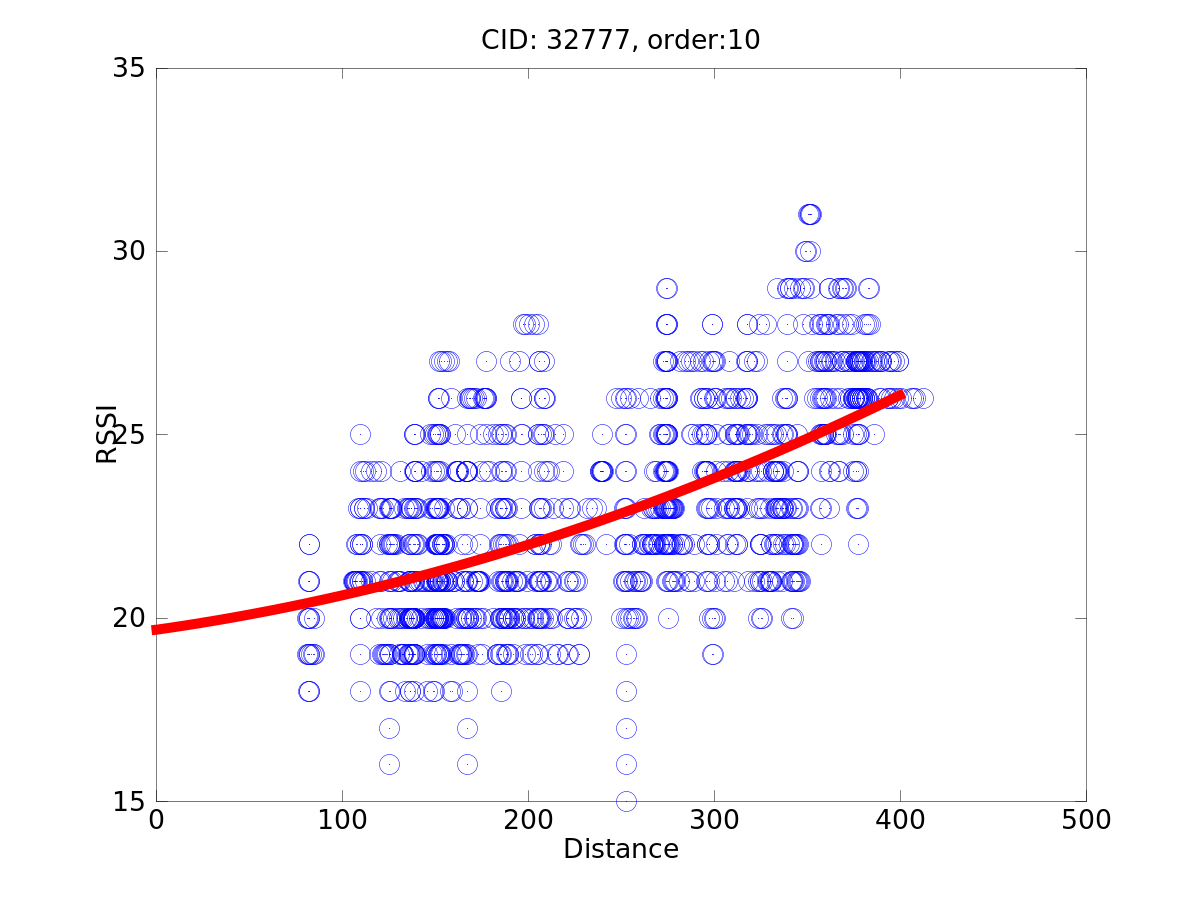
\includegraphics[width=1\textwidth]{cell32777inter10-contrast.png}

			Maximal degree of a polynomial: 10
		\column{0.45\textwidth}
			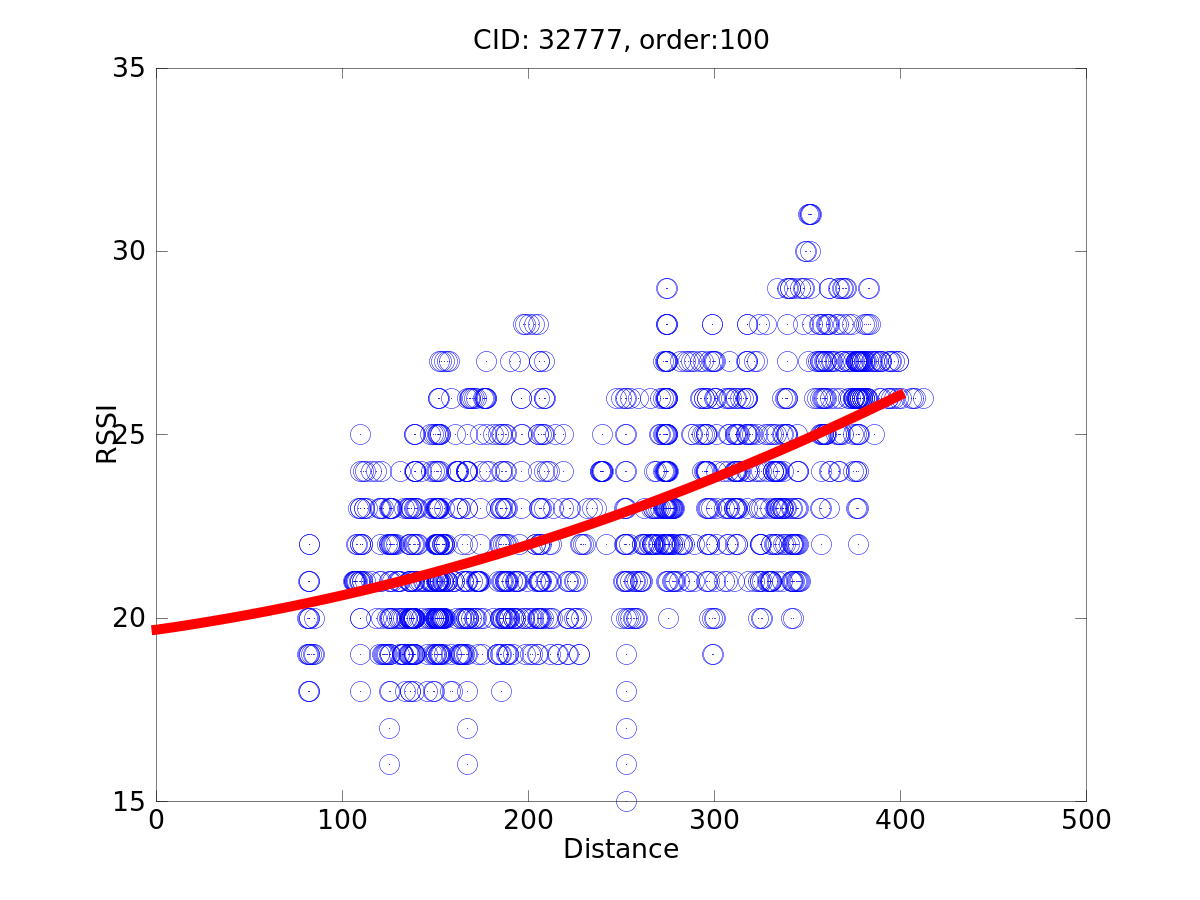
\includegraphics[width=1\textwidth]{cell32777inter100-contrast.png}
			
			Maximal degree of a polynomial: 100
	\end{columns}
\end{figure}
}

\frame{
	\frametitle{Conclusion}
	\begin{enumerate}
		\item
			The new method works;
		\item
			Its precision is better than that of triangulation;
		\item
			Its precision is worse than that of GPS;
		\item
			Additional improvements are required and possible.
	\end{enumerate}
}
\frame{\titlepage}

\appendix
\newcounter{finalframe}
\setcounter{finalframe}{\value{framenumber}}
\setbeamertemplate{footline}
{
  \leavevmode%
  \hbox{\large%
  \begin{beamercolorbox}[wd=.3\paperwidth,ht=2.25ex,dp=1ex,center]{author in head/foot}%
    \usebeamerfont{author in head/foot}\insertshortauthor
  \end{beamercolorbox}%
  \begin{beamercolorbox}[wd=.59\paperwidth,ht=2.25ex,dp=1ex,center]{title in head/foot}%
    \usebeamerfont{title in head/foot}\insertshorttitle
  \end{beamercolorbox}%
  \begin{beamercolorbox}[wd=.11\paperwidth,ht=2.25ex,dp=1ex,right]{date in head/foot}%
	\insertframenumber\hspace*{2ex}
  \end{beamercolorbox}}%
  \vskip0pt%
}

\frame{
	\frametitle{Threads of the server-side}
	\centerline{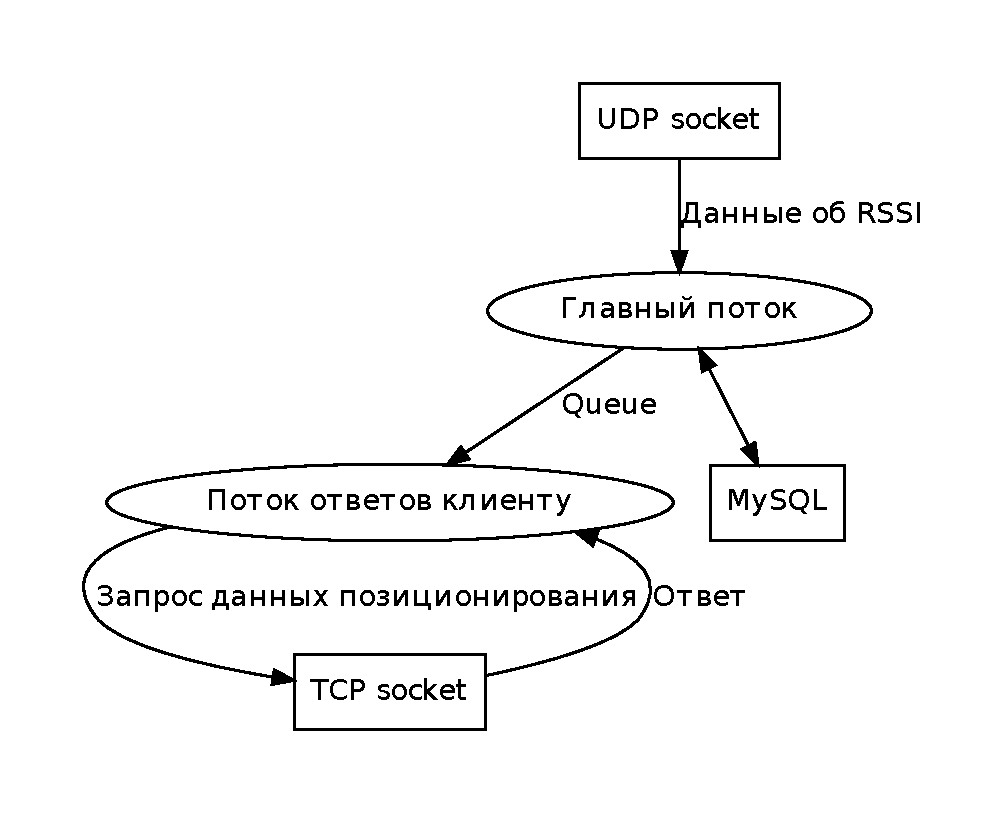
\includegraphics[height=0.8\textheight]{server-threads.pdf}}
}

\frame{
	\frametitle{Collecting data mode}
	\centerline{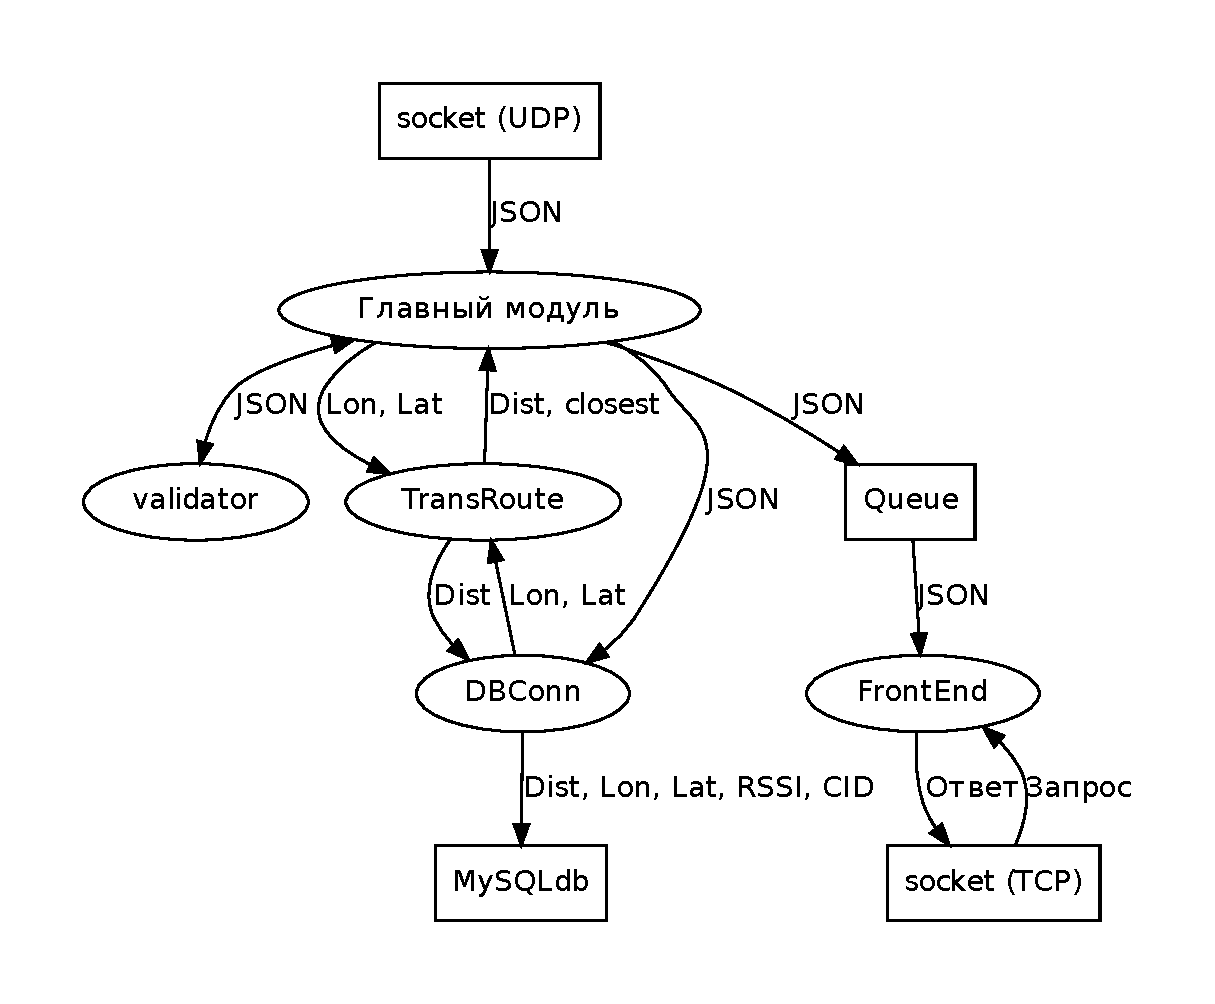
\includegraphics[height=0.8\textheight]{server-collect-dataflow.pdf}}
}

\frame{
	\frametitle{Positioning mode}
	\centerline{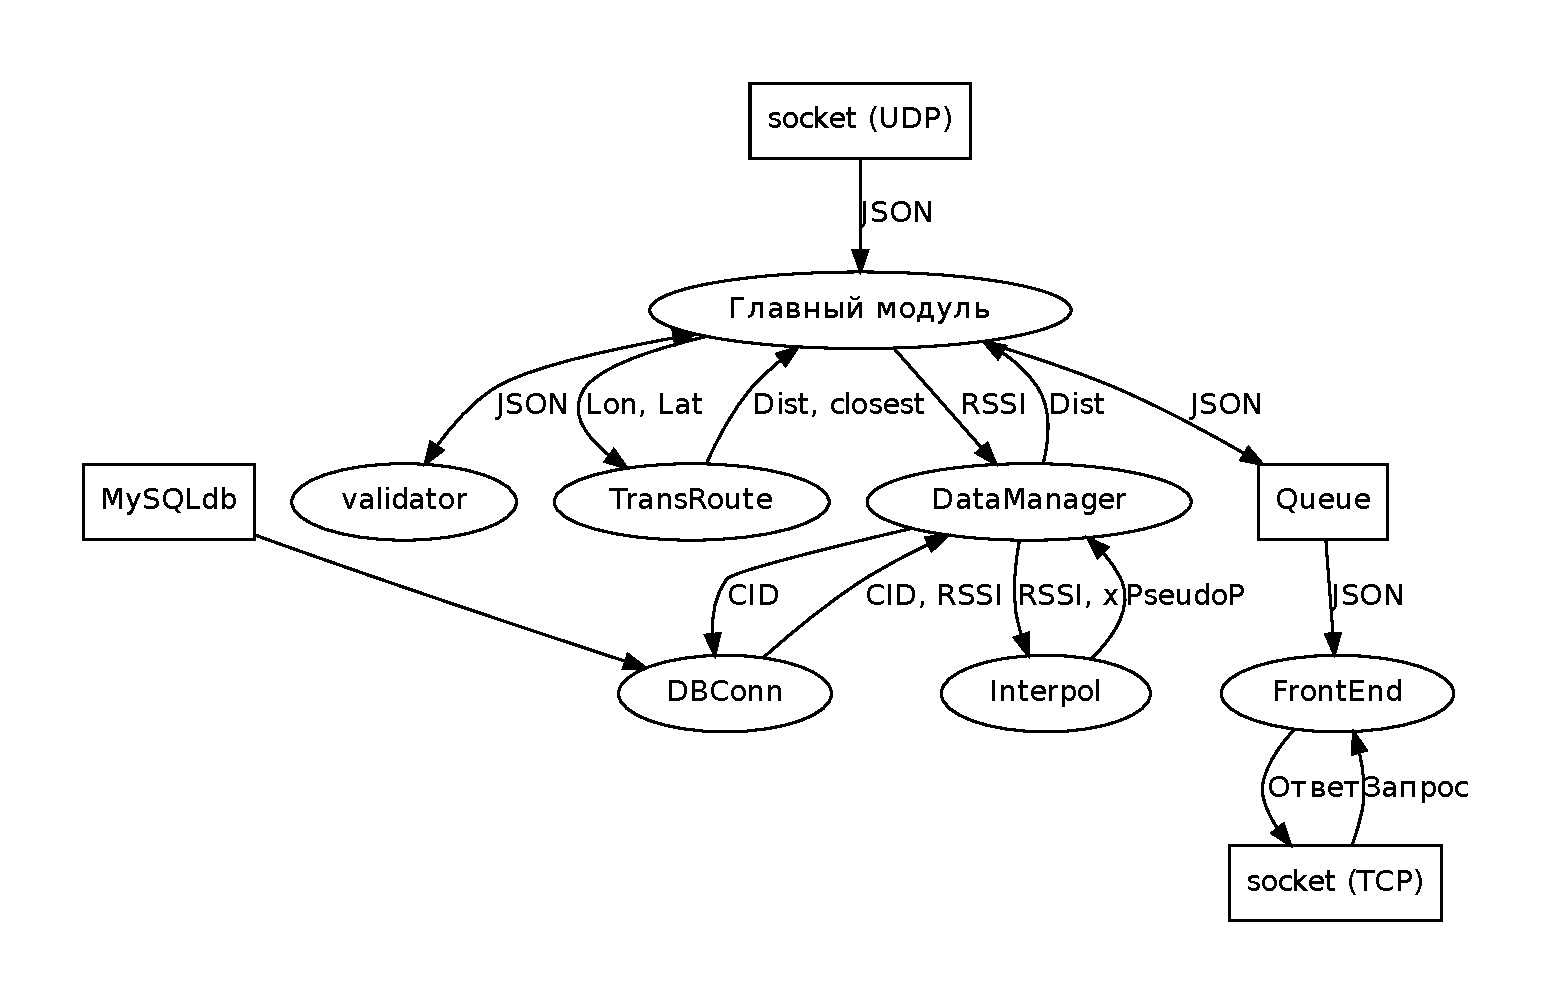
\includegraphics[height=0.8\textheight]{server-perform-dataflow.pdf}}
}

\frame{
	\frametitle{Mobile application}
	\centerline{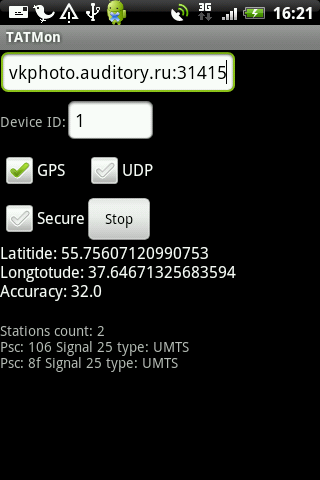
\includegraphics[height=0.8\textheight]{TATMon-android.png}}
}


\begin{frame}[fragile]
	\frametitle{Example of a message}
	\begin{lstlisting}
{	"GSM":{
		"cellcount":2, 
		"cells":[
				{"CID":11531, "Psc":-1, "RSSI":26, "type":"EDGE"}, 
				{"CID":32779, "Psc":-1, "RSSI":22, "type":"EDGE"}
			]
		},
	"GPS": {
			"lng":37.64814019203186,
			"ltd":55.75437605381012,
			"acc":24.0
		}}
	\end{lstlisting}
\end{frame}

\frame{
	\frametitle{Algorithm input}
	\begin{equation}
		data = \begin{pmatrix}
			Dist_0 & RSSI_0 \\
			Dist_1 & RSSI_1 \\
			\vdots & \vdots \\
    Dist_{len(data)-1} & RSSI_{len(data)-1}
		\end{pmatrix}
		\nonumber
		\label{eq:data-create-vars}
	\end{equation}
}

\frame{
	\frametitle{Creating variables}
		\begin{equation}
			self.X = \begin{pmatrix}
				1 & Dist_0 & Dist_0^2 & \cdots & Dist_0^{order} \\
				1 & Dist_1 & Dist_1^2 & \cdots & Dist_1^{order} \\
      \vdots & \vdots & \vdots & \vdots & \vdots \\
				       1 & Dist_{len(data)-1} & Dist_{len(data)-1}^2 & \cdots & Dist_{len(data)-1}^{order}
			\end{pmatrix}
			\label{eq:self-x-create-vars}
			\nonumber
		\end{equation}

		\begin{equation}
			self.Y = \begin{pmatrix}
				RSSI_0 \\
				RSSI_1 \\
				\vdots \\
				RSSI_{len(data)-1}
			\end{pmatrix}
			\nonumber
			\label{eq:self-y-create-vars}
		\end{equation}
}

\begin{frame}[fragile]
	\frametitle{Normal equations}
	\begin{equation}
		self.theta = (self.X^\intercal \cdot self.X)^{+} \cdot self.X^\intercal \cdot self.Y
		\nonumber
		\label{eq:solve-theta}
	\end{equation}
\begin{lstlisting}
def solve_theta(self):
    self.theta = numpy.transpose(self.X)
    self.theta = numpy.dot(self.theta, self.X)
    self.theta = numpy.linalg.pinv(self.theta)
    self.theta = numpy.dot(self.theta,\
        numpy.transpose(self.X))
    self.theta = numpy.dot(self.theta, self.Y)
\end{lstlisting}
\end{frame}
\setcounter{framenumber}{\value{finalframe}}

\end{document}


